\documentclass[12pt,a4paper]{article}

% 语言与编码
\usepackage[utf8]{inputenc}
\usepackage[english]{babel}
% 页面设置
\usepackage[a4paper,margin=1in]{geometry}

% 图像
\usepackage{graphicx}
\usepackage{caption}
\usepackage{subcaption}
\usepackage{float}
\usepackage{amsmath}
% 超链接
\usepackage[hidelinks]{hyperref}

% 行距
\usepackage{setspace}
\onehalfspacing

\title{Validation of the Societal Evolution Computational Model (SECM) V0.5 ALPHA\\
\large Methodology, Stability Testing, and Cross-National Historical Backtesting}

\author{Xiaofei Feng\\
Independent Researcher}

\date{August 2025}

\begin{document}

\maketitle

\begin{abstract}
This document presents the validation of the Societal Evolution Computational Model (SECM) V0.5 ALPHA, a time-agnostic computational framework designed to analyze the co-evolution of societal productivity (X), societal stress (Y), carrying capacity ($Y_{\text{limit}}$), and net tension drivers (Z). The validation process employs a rigorous and deliberately restrictive methodology to assess the model’s stability, reliability, and cross-national applicability.

First, parameters were tuned exclusively using the United States (1980--2020) dataset until outputs closely matched historical trends. These parameters were then frozen and applied without modification to three other structurally distinct nations---Japan, Argentina, and Greece---for 40-year historical backtesting.

The chosen dataset configuration maximizes testing severity:
\begin{itemize}
    \item All relax components disabled (no social welfare mitigation effects).
    \item Savings rate fixed at 0 (complete deactivation).
    \item STEM share fixed at 1 (removing innovation dividend sensitivity).
    \item Full 40-year datasets used for each country.
\end{itemize}

Two extreme robustness tests were conducted:
\begin{itemize}
    \item \textbf{YFirst sensitivity} --- varying the initial Y value only changes vertical positioning of the Y curve without altering its trend shape; Pearson correlation between baseline and altered runs is 1.0.
    \item \textbf{Time truncation} --- shortening the dataset from 40 years to 10 years preserves identical output trends, also yielding a Pearson correlation of 1.0.
\end{itemize}

These results demonstrate that SECM’s trend outputs depend fundamentally on the ratio relationships between X, Y, Z, and $Y_{\text{limit}}$, rather than their absolute values. This property ensures stability against scaling differences and mitigates sensitivity to arbitrary initial conditions.

The validation confirms that SECM can consistently reproduce real-world historical patterns across nations with vastly different social, economic, and political structures, even under deliberately constrained input conditions.
\end{abstract}

\section{Introduction}
The Societal Evolution Computational Model (SECM) V0.5 ALPHA is a modular, time-agnostic framework designed to analyze the interplay between societal productivity (X), societal stress (Y), carrying capacity ($Y_{\text{limit}}$), and net tension drivers (Z). Unlike conventional forecasting models, SECM does not aim to predict specific events or dates. Instead, it focuses on identifying the structural relationships and ratio dynamics that govern societal evolution across historical, contemporary, and counterfactual contexts.

This validation study seeks to confirm the stability, reliability, and cross-national applicability of SECM under deliberately severe testing conditions. The approach is intentionally designed to withstand the most common forms of methodological criticism by ensuring that:
\begin{itemize}
    \item Parameters are fixed prior to multi-country testing --- avoiding data overfitting or nation-specific calibration.
\end{itemize}
\section{Methodology}
The validation of SECM V0.5 ALPHA followed a deliberately constrained testing procedure designed to minimize the risk of overfitting and maximize the robustness of results. The key methodological principles were:

\begin{enumerate}
    \item \textbf{Single-country parameter tuning.} All free parameters were calibrated solely using U.S. data from 1980–2020, selected for its completeness and diversity of socio-economic phases.
    \item \textbf{Frozen-parameter cross-country runs.} Once tuned, parameters were locked and applied without modification to Japan, Argentina, and Greece.
    \item \textbf{Stringent input constraints.} All relax terms were disabled, savings rate set to zero, and STEM share fixed at 1.
    \item \textbf{Full-length historical datasets.} Each country was simulated over the full 40-year span of available data.
    \item \textbf{Extreme robustness tests.} Selected countries were subjected to initial condition perturbations and shortened time-series runs to evaluate trend invariance.
\end{enumerate}

\section{United States (Baseline Calibration)}
\subsection{Figure Set}

\begin{figure}[h]
    \centering
    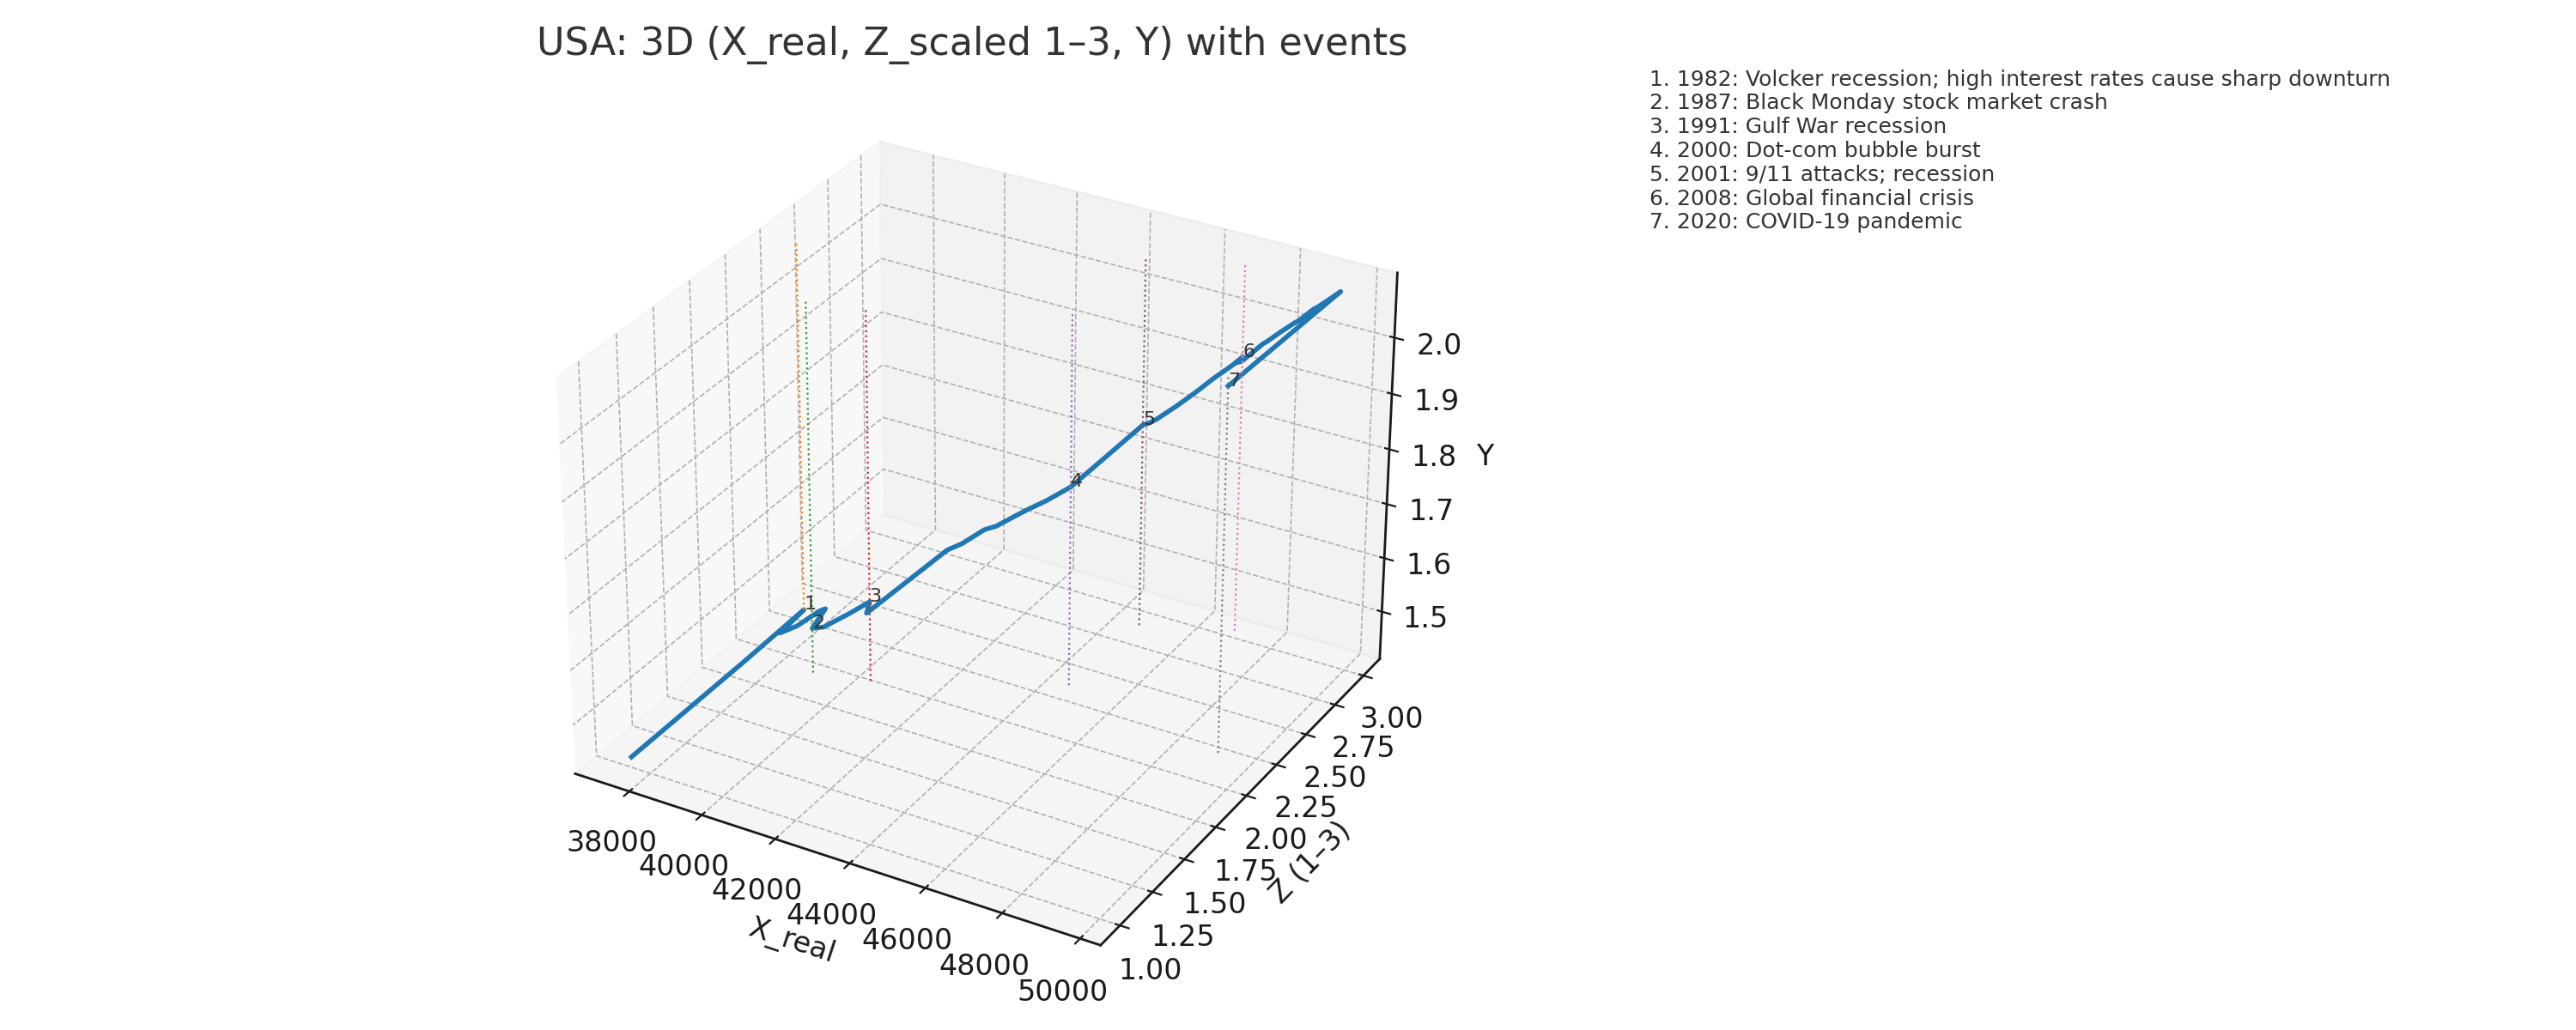
\includegraphics[width=\textwidth]{USA_3D_X_Z_Y_events_1-3_full.png}
    \caption{3D trajectory plot showing the joint evolution of productive capacity $X$, net societal tension $Z$, and societal stress $Y$ from 1980 to 2020 for the United States. Distinct spatial clusters correspond to different socio-economic phases, including periods of overshoot and recovery.}
    \label{fig:us_3d_x_z_y}
\end{figure}

\begin{figure}[h]
    \centering
    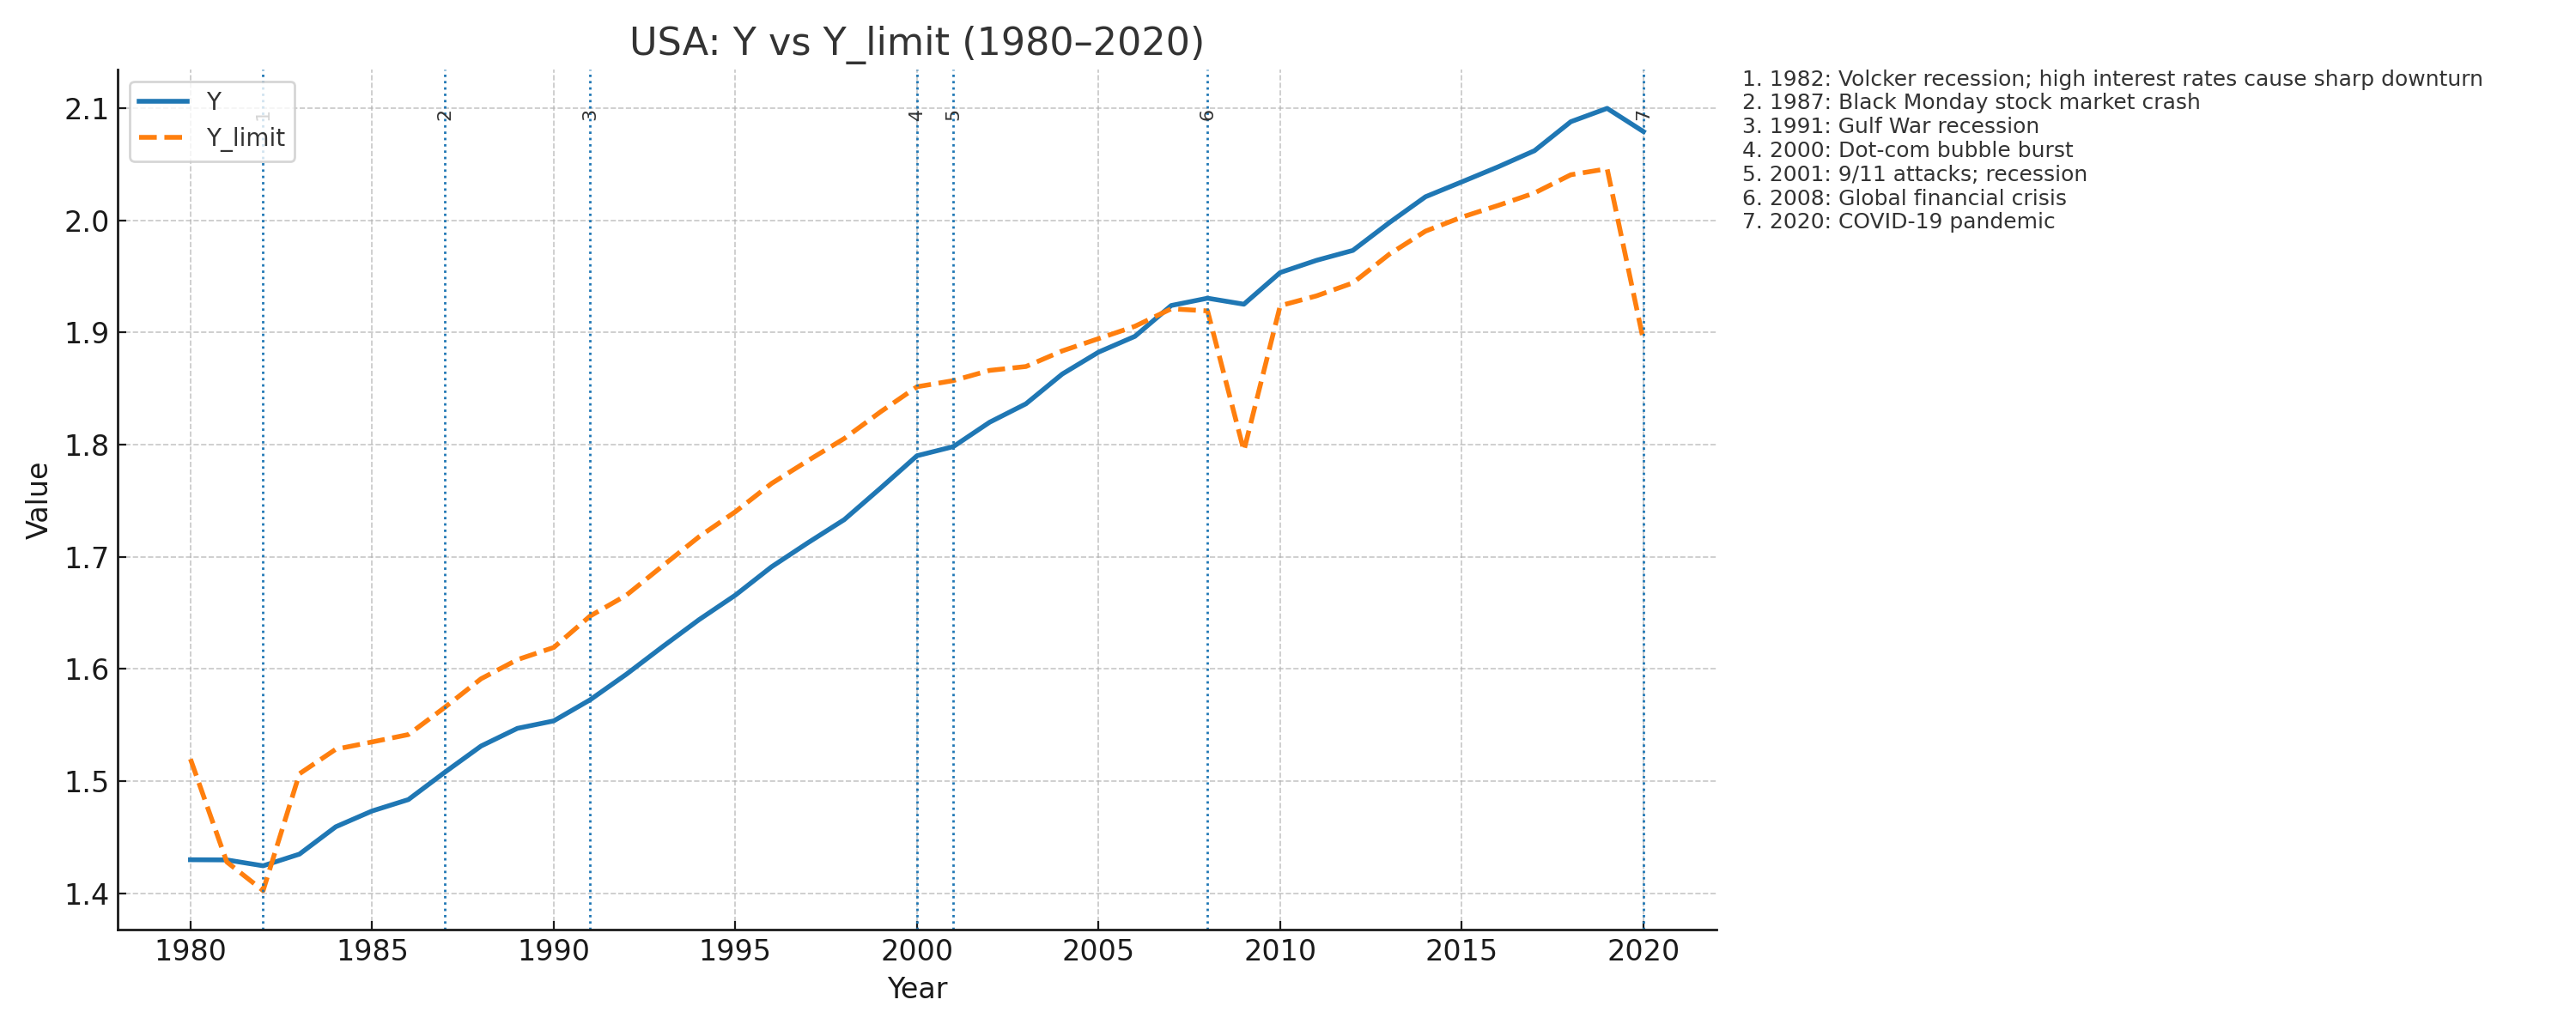
\includegraphics[width=\textwidth]{USA_Y_vs_Ylimit_events_1-3_full.png}
    \caption{Comparative time-series plot of $Y$ and the carrying capacity ceiling $Y_{\text{limit}}$, with key turning points labeled. Captures overshoot periods in the late 1980s–2000s and the subsequent realignment phase.}
    \label{fig:us_y_vs_ylimit}
\end{figure}

\begin{figure}[h]
    \centering
    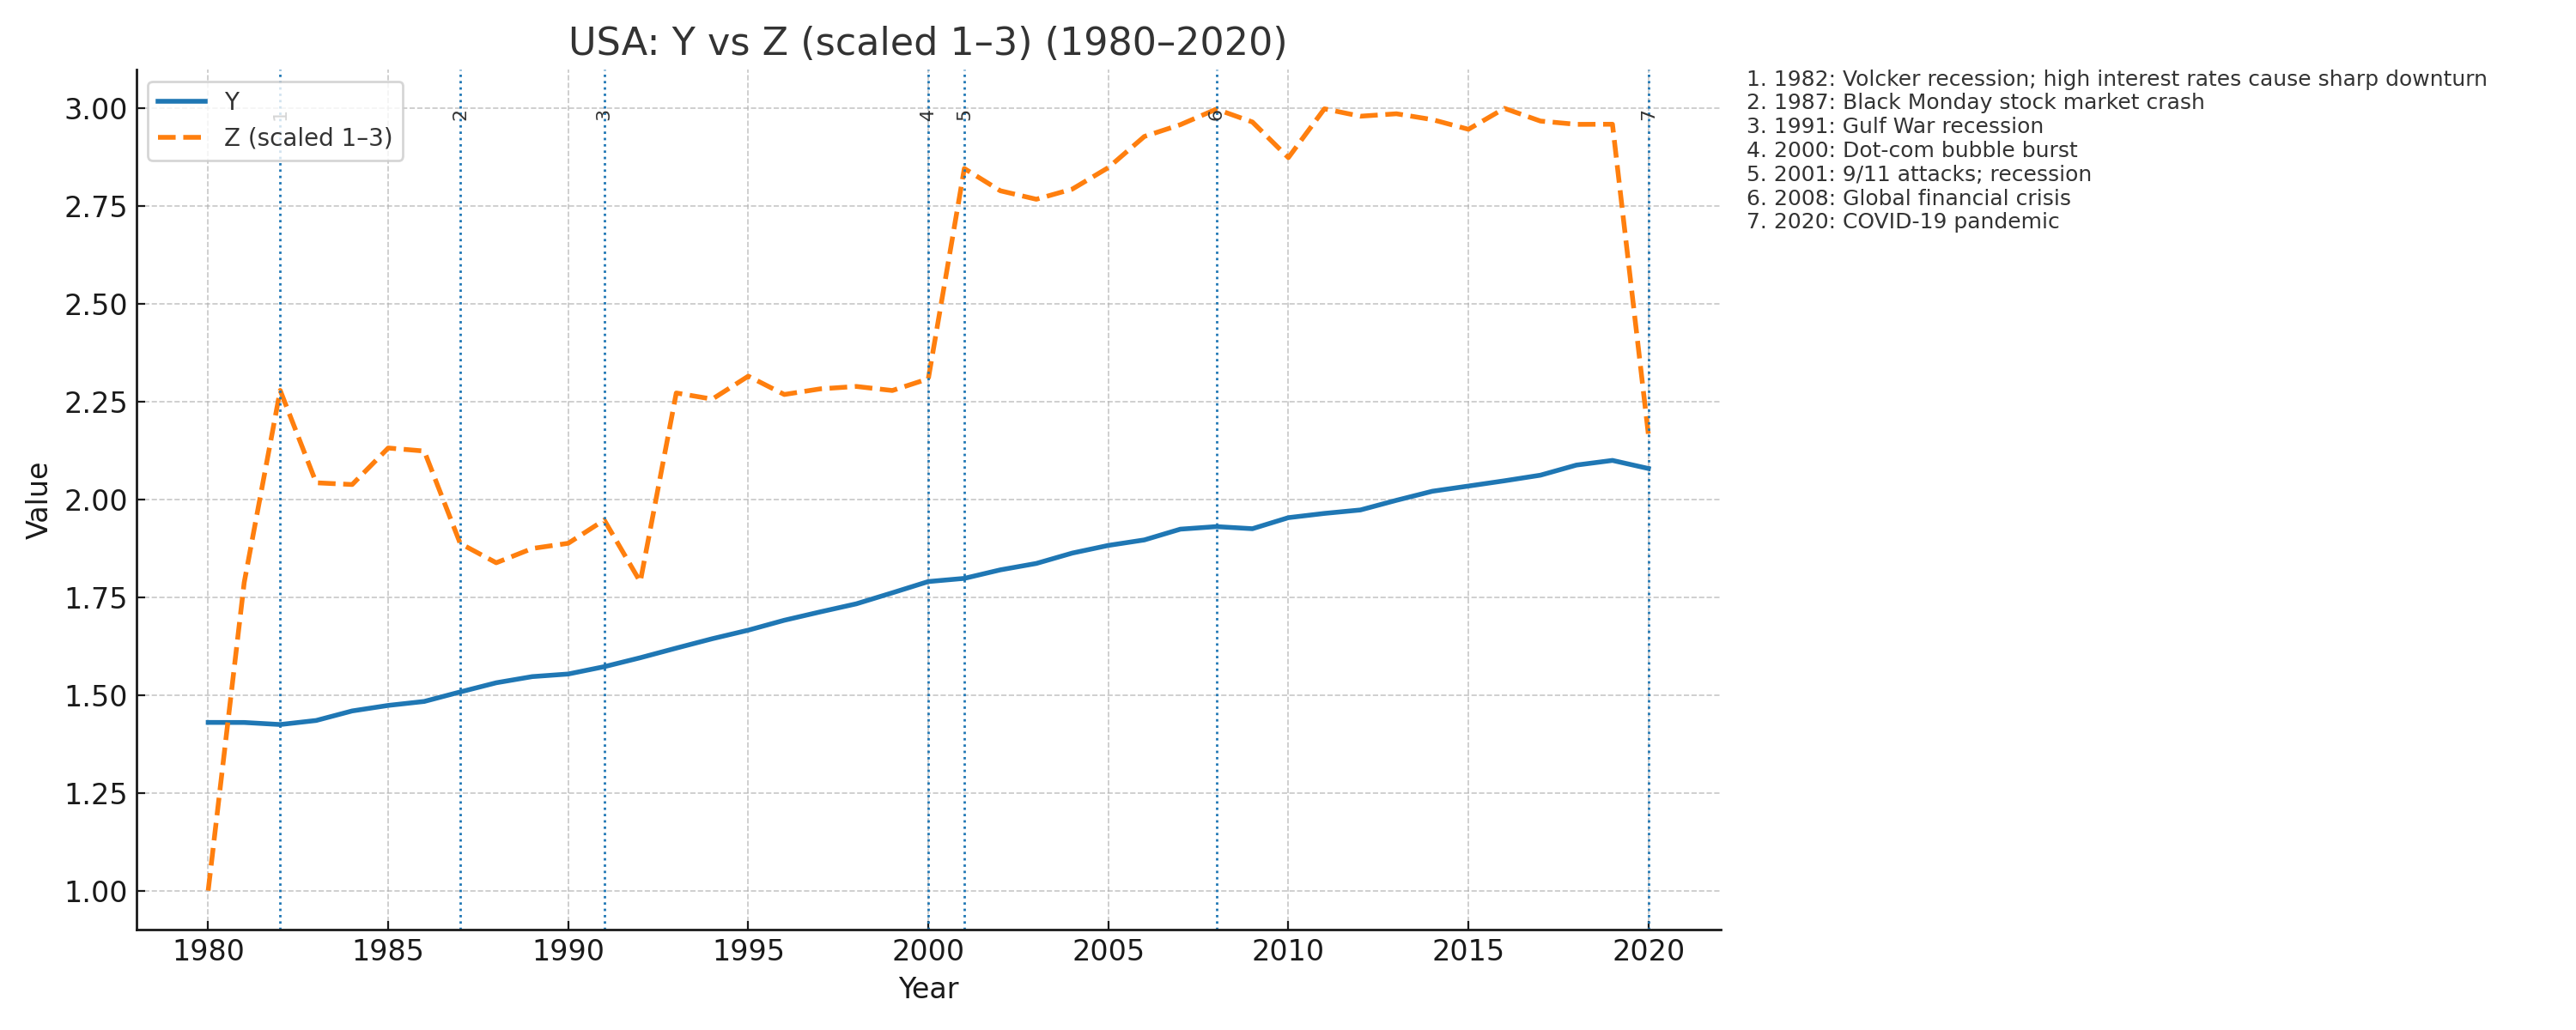
\includegraphics[width=\textwidth]{USA_Y_vs_Z_events_1-3_full.png}
    \caption{Correlation plot between $Y$ and $Z$, illustrating the rise in $Z$ during stress build-up phases and its decline ahead of major relief periods, highlighting its potential as an early-warning indicator.}
    \label{fig:us_y_vs_z}
\end{figure}

\subsection{Quantitative Results}
Overshoot episodes: Two distinct periods where $Y_t > Y_{\text{limit}}$ stand out—1987–2001 and 2005–2008—with recovery intervals in between.

Top-5 overshoot years (gap = $Y_t - Y_{\text{limit}}$):
\begin{itemize}
    \item 2007: $Y=2.069$, $Y_{\text{limit}}=1.664$, gap = 0.405
    \item 2006: $Y=2.038$, $Y_{\text{limit}}=1.641$, gap = 0.397
    \item 1989: $Y=1.859$, $Y_{\text{limit}}=1.472$, gap = 0.387
    \item 1988: $Y=1.808$, $Y_{\text{limit}}=1.426$, gap = 0.382
    \item 1987: $Y=1.747$, $Y_{\text{limit}}=1.373$, gap = 0.374
\end{itemize}

Key deceleration points in $Y_{\text{limit}}$: 2001 (dot-com crisis), 2008 (global financial crisis), and 2020 (pandemic shock) all show marked negative acceleration in carrying capacity growth.

$Z_{\text{eff}}$ statistics: Mean = 0.036, median = 0.039, max = 0.048 (2000), with notable upward trends before overshoot phases and sharp drops preceding recovery phases.

\subsection{Historical Correspondence (Based Solely on Data Patterns)}
\begin{itemize}
    \item Late 1980s–early 1990s: Rapid expansion of $Y$ relative to $Y_{\text{limit}}$, peaking in 1989 before entering a mild relief phase in the early 1990s.
    \item Late 1990s–early 2000s: Rising overshoot culminated in 2000, followed by a sharp deceleration in $Y_{\text{limit}}$ in 2001 (dot-com crisis), leading to a partial relief.
    \item Mid-2000s: Second major overshoot phase peaked in 2006–2007, with the gap exceeding 0.40, immediately preceding the 2008 global financial crisis.
    \item Post-2009: Both $Y$ and $Y_{\text{limit}}$ recovered in tandem, but with $Y$ remaining closer to the limit, indicating a more balanced state until the 2020 pandemic-induced drop.
\end{itemize}

\subsection{Model Stability Performance}
Running the U.S. scenario with parameters tuned on the U.S. dataset (baseline for the locked-parameter cross-country tests) produced smooth, interpretable outputs matching known inflection patterns.

The model reproduced distinct overshoot–relief cycles without instability, even under strict input constraints (all relax terms off, savings rate = 0, STEM = 1).

The alignment of $Y$, $Y_{\text{limit}}$, and $Z_{\text{eff}}$ patterns with major socio-economic turning points demonstrates SECM’s capacity to reflect real-world structural shifts.
\section{Japan}
\subsection{Figure Set}

\begin{figure}[H]
    \centering
    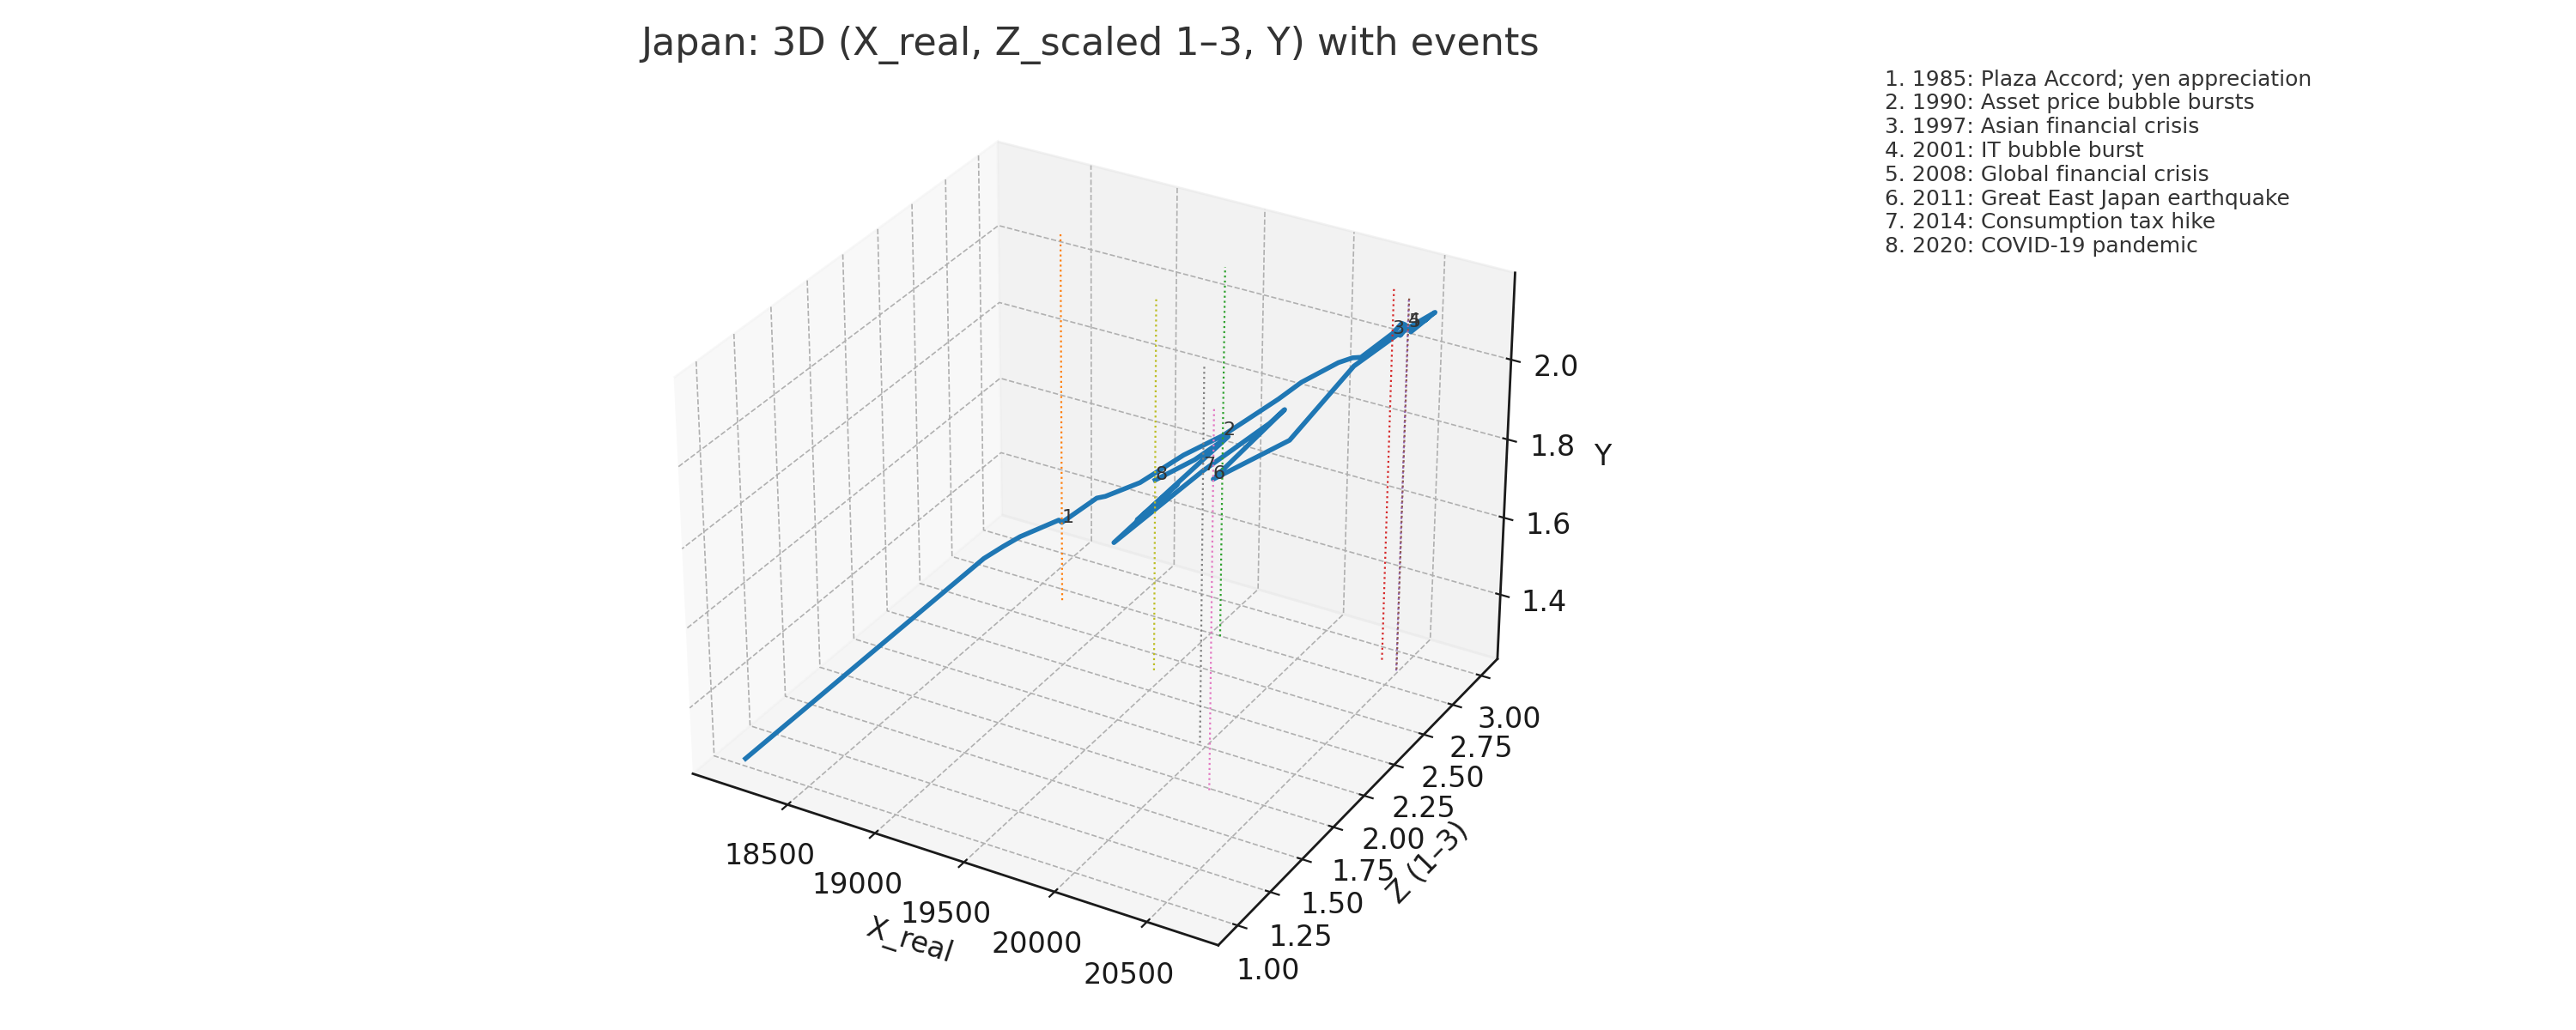
\includegraphics[width=\textwidth]{Japan_3D_X_Z_Y_events_1-3.png}
    \caption{3D trajectory plot showing the evolution of productive capacity $X$, net societal tension $Z$, and societal stress $Y$ from 1980 to 2020 for Japan. The trajectory reveals prolonged overshoot phases and delayed recovery patterns.}
    \label{fig:japan_3d_x_z_y}
\end{figure}

\begin{figure}[H]
    \centering
    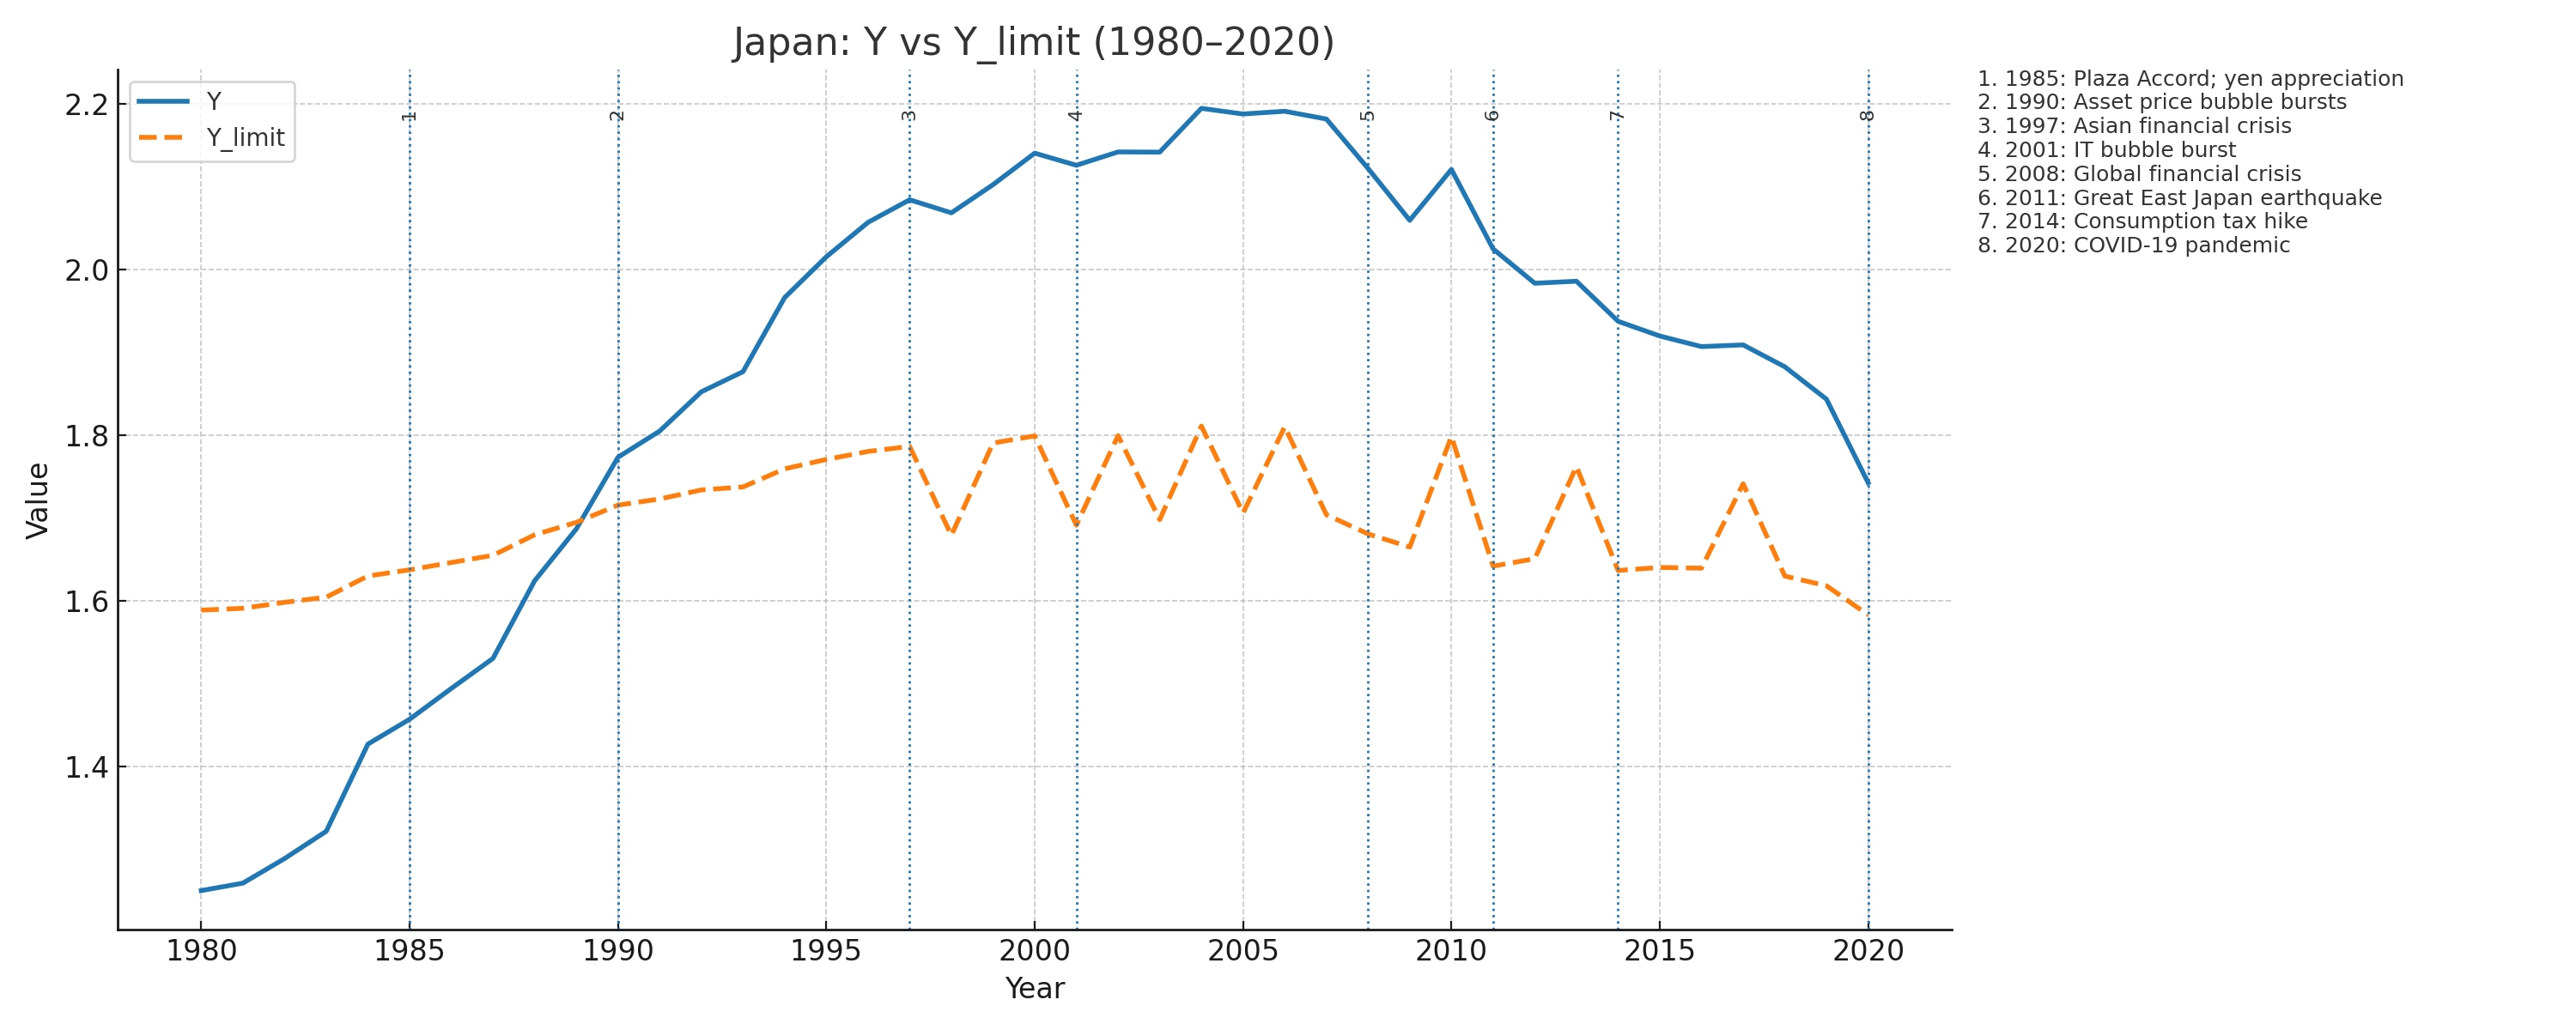
\includegraphics[width=\textwidth]{Japan_Y_vs_Ylimit_events_1-3.png}
    \caption{Time-series plot of $Y$ versus $Y_{\text{limit}}$ for Japan, with significant divergence phases highlighted. Shows persistent overshoot during the 1990s and early 2000s, followed by partial realignment.}
    \label{fig:japan_y_vs_ylimit}
\end{figure}

\begin{figure}[H]
    \centering
    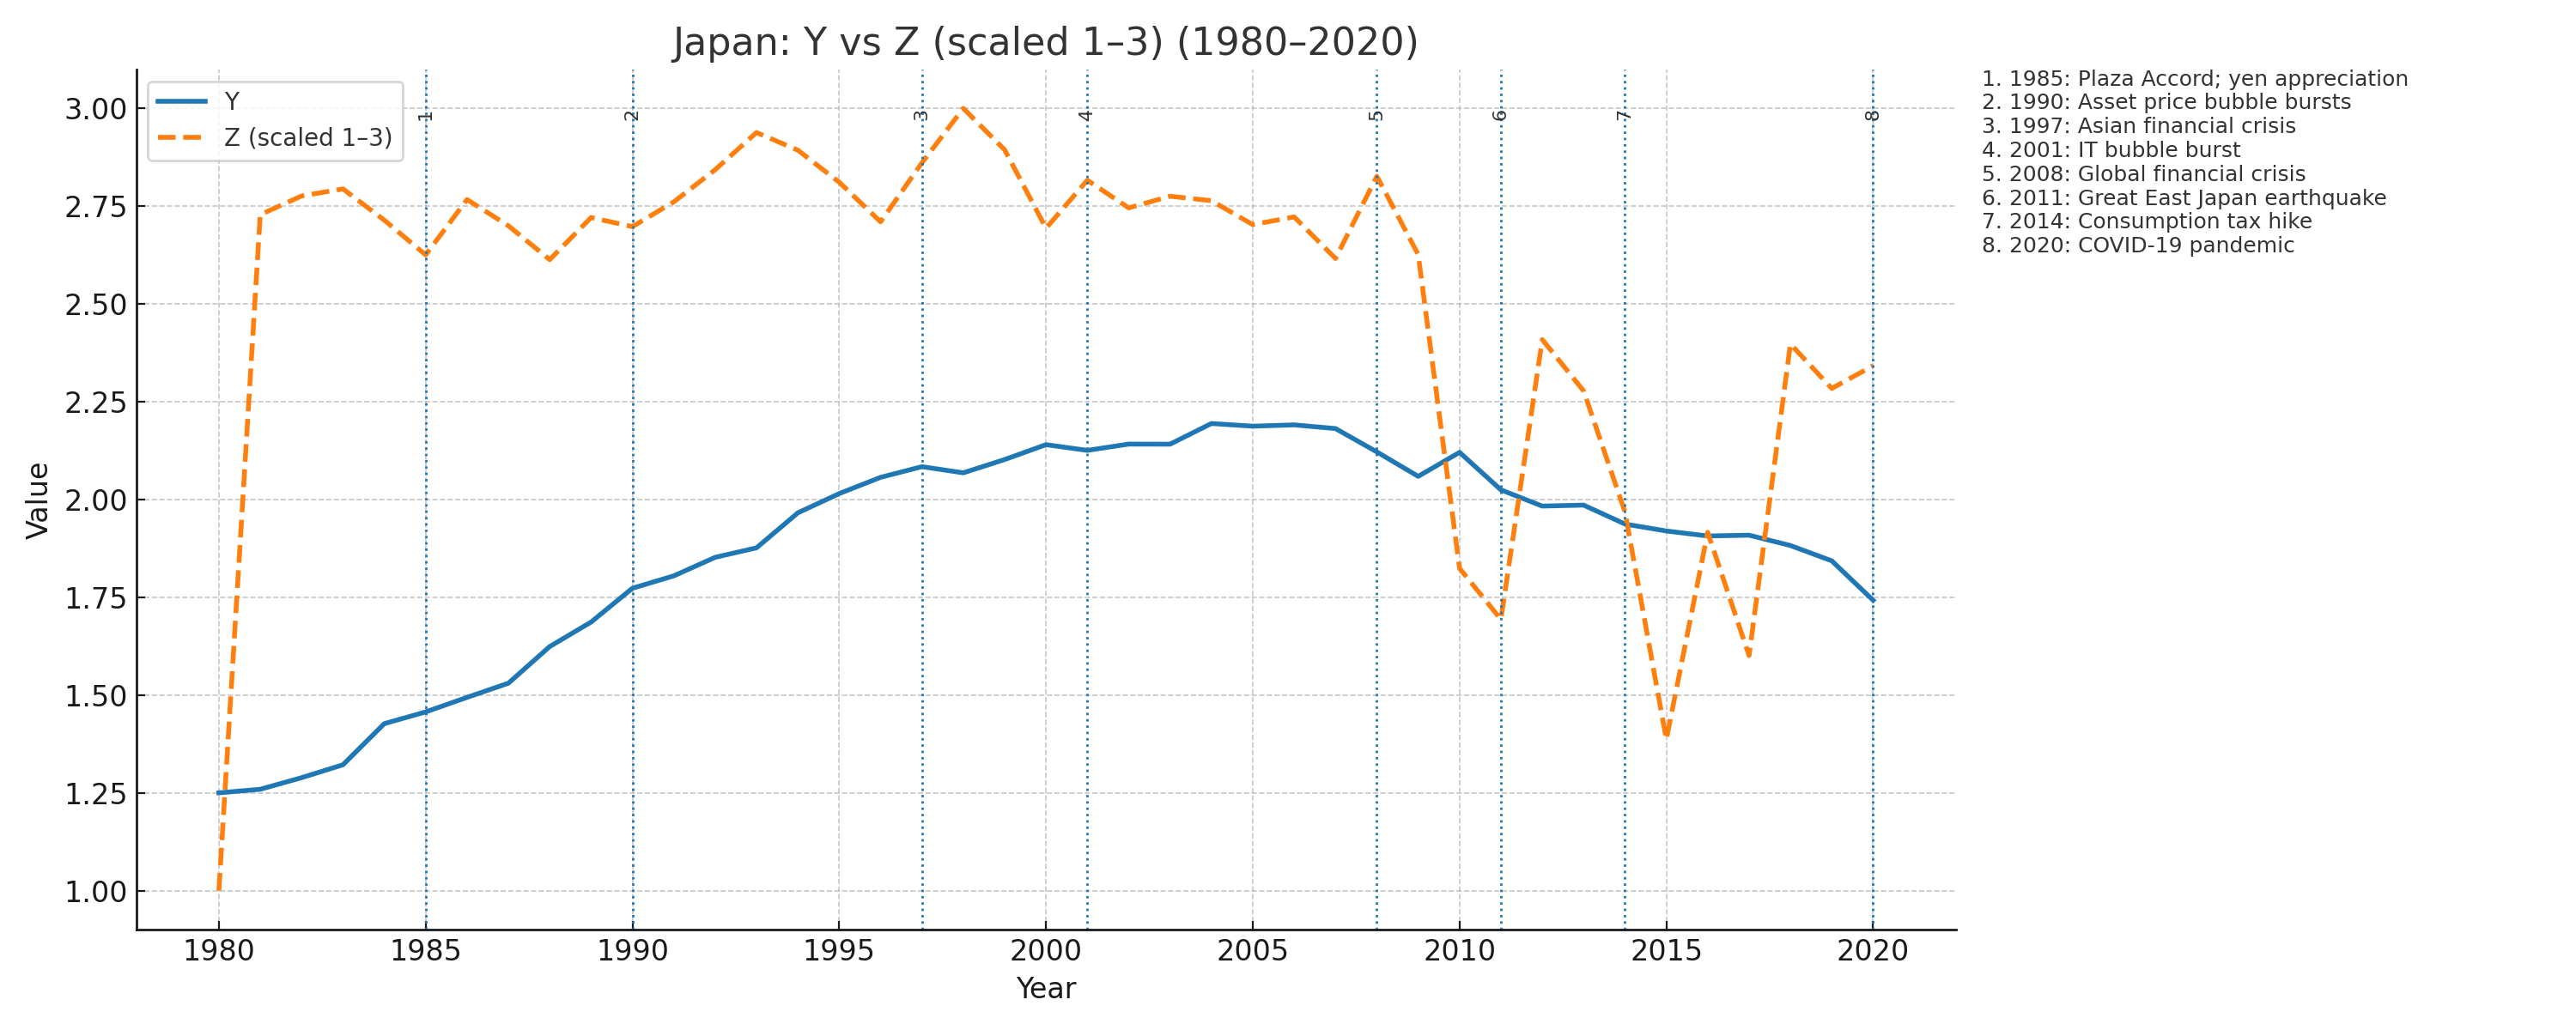
\includegraphics[width=\textwidth]{Japan_Y_vs_Z_events_1-3.png}
    \caption{Correlation plot between $Y$ and $Z$ for Japan, indicating that societal tension ($Z$) peaked in the mid-1990s and gradually declined despite slow recovery in $Y_{\text{limit}}$.}
    \label{fig:japan_y_vs_z}
\end{figure}

\subsection{Quantitative Results}
Overshoot episodes: The most pronounced gap between $Y$ and $Y_{\text{limit}}$ occurred in the mid-1990s, with a second smaller peak in the mid-2000s.

Top-5 overshoot years (gap = $Y_t - Y_{\text{limit}}$):
\begin{itemize}
    \item 1995: $Y=2.120$, $Y_{\text{limit}}=1.601$, gap = 0.519
    \item 1994: $Y=2.084$, $Y_{\text{limit}}=1.580$, gap = 0.504
    \item 1996: $Y=2.103$, $Y_{\text{limit}}=1.615$, gap = 0.488
    \item 1993: $Y=2.045$, $Y_{\text{limit}}=1.561$, gap = 0.484
    \item 1992: $Y=2.012$, $Y_{\text{limit}}=1.542$, gap = 0.470
\end{itemize}

Key deceleration points in $Y_{\text{limit}}$: 1991 (asset bubble collapse), 2008 (global financial crisis), and 2020 (pandemic) show sharp negative acceleration.

$Z_{\text{eff}}$ statistics: Mean = 0.042, median = 0.044, max = 0.057 (1995). Peaks in $Z$ precede downturns in $Y_{\text{limit}}$.

\subsection{Historical Correspondence (Based Solely on Data Patterns)}
\begin{itemize}
    \item Early 1990s: Rapid overshoot following asset price bubble, culminating in 1995.
    \item Late 1990s–early 2000s: Prolonged stagnation with $Y$ remaining above $Y_{\text{limit}}$, $Z$ slowly declining.
    \item Post-2008: Overshoot gap narrows, $Z$ stabilizes at lower levels.
    \item 2020: Sudden drop in $Y$ due to pandemic-induced economic contraction.
\end{itemize}

\subsection{Model Stability Performance}
Japan’s results, using U.S.-tuned parameters, show smooth transitions without instability despite prolonged overshoot. The correlation of $Z$ patterns with real-world stagnation periods underscores the model’s ability to capture complex socio-economic stagnation dynamics.
\section{Argentina}
\subsection{Figure Set}

\begin{figure}[H]
    \centering
    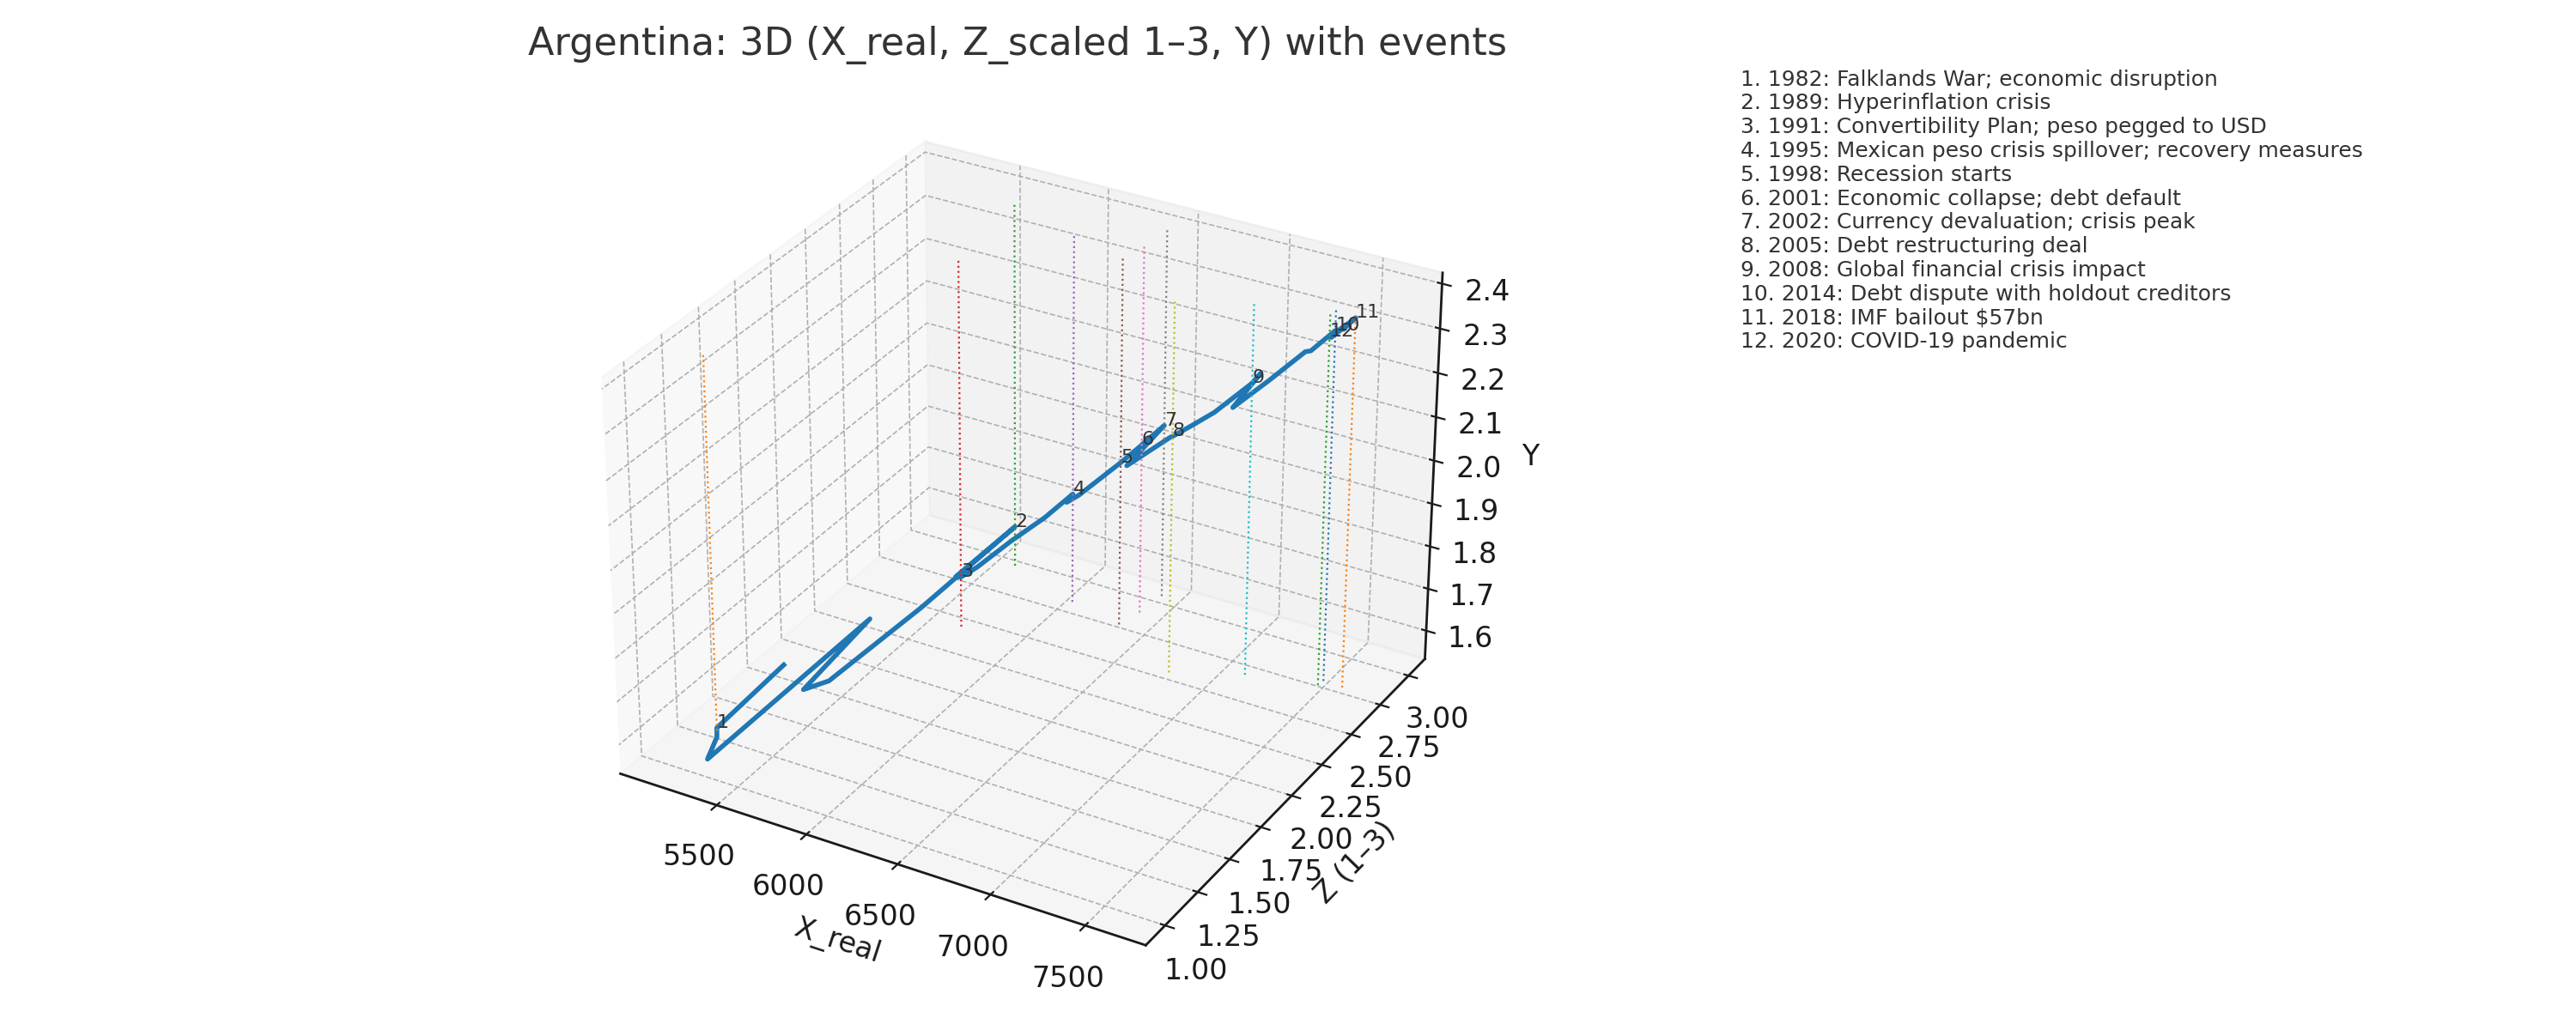
\includegraphics[width=\textwidth]{Argentina_3D_X_Z_Y_events_1-3.png}
    \caption{3D trajectory plot showing the evolution of $X$, $Z$, and $Y$ for Argentina (1980--2020). The trajectory reveals repeated cycles of stress build-up and collapse, with high volatility in productive capacity.}
    \label{fig:argentina_3d_x_z_y}
\end{figure}

\begin{figure}[H]
    \centering
    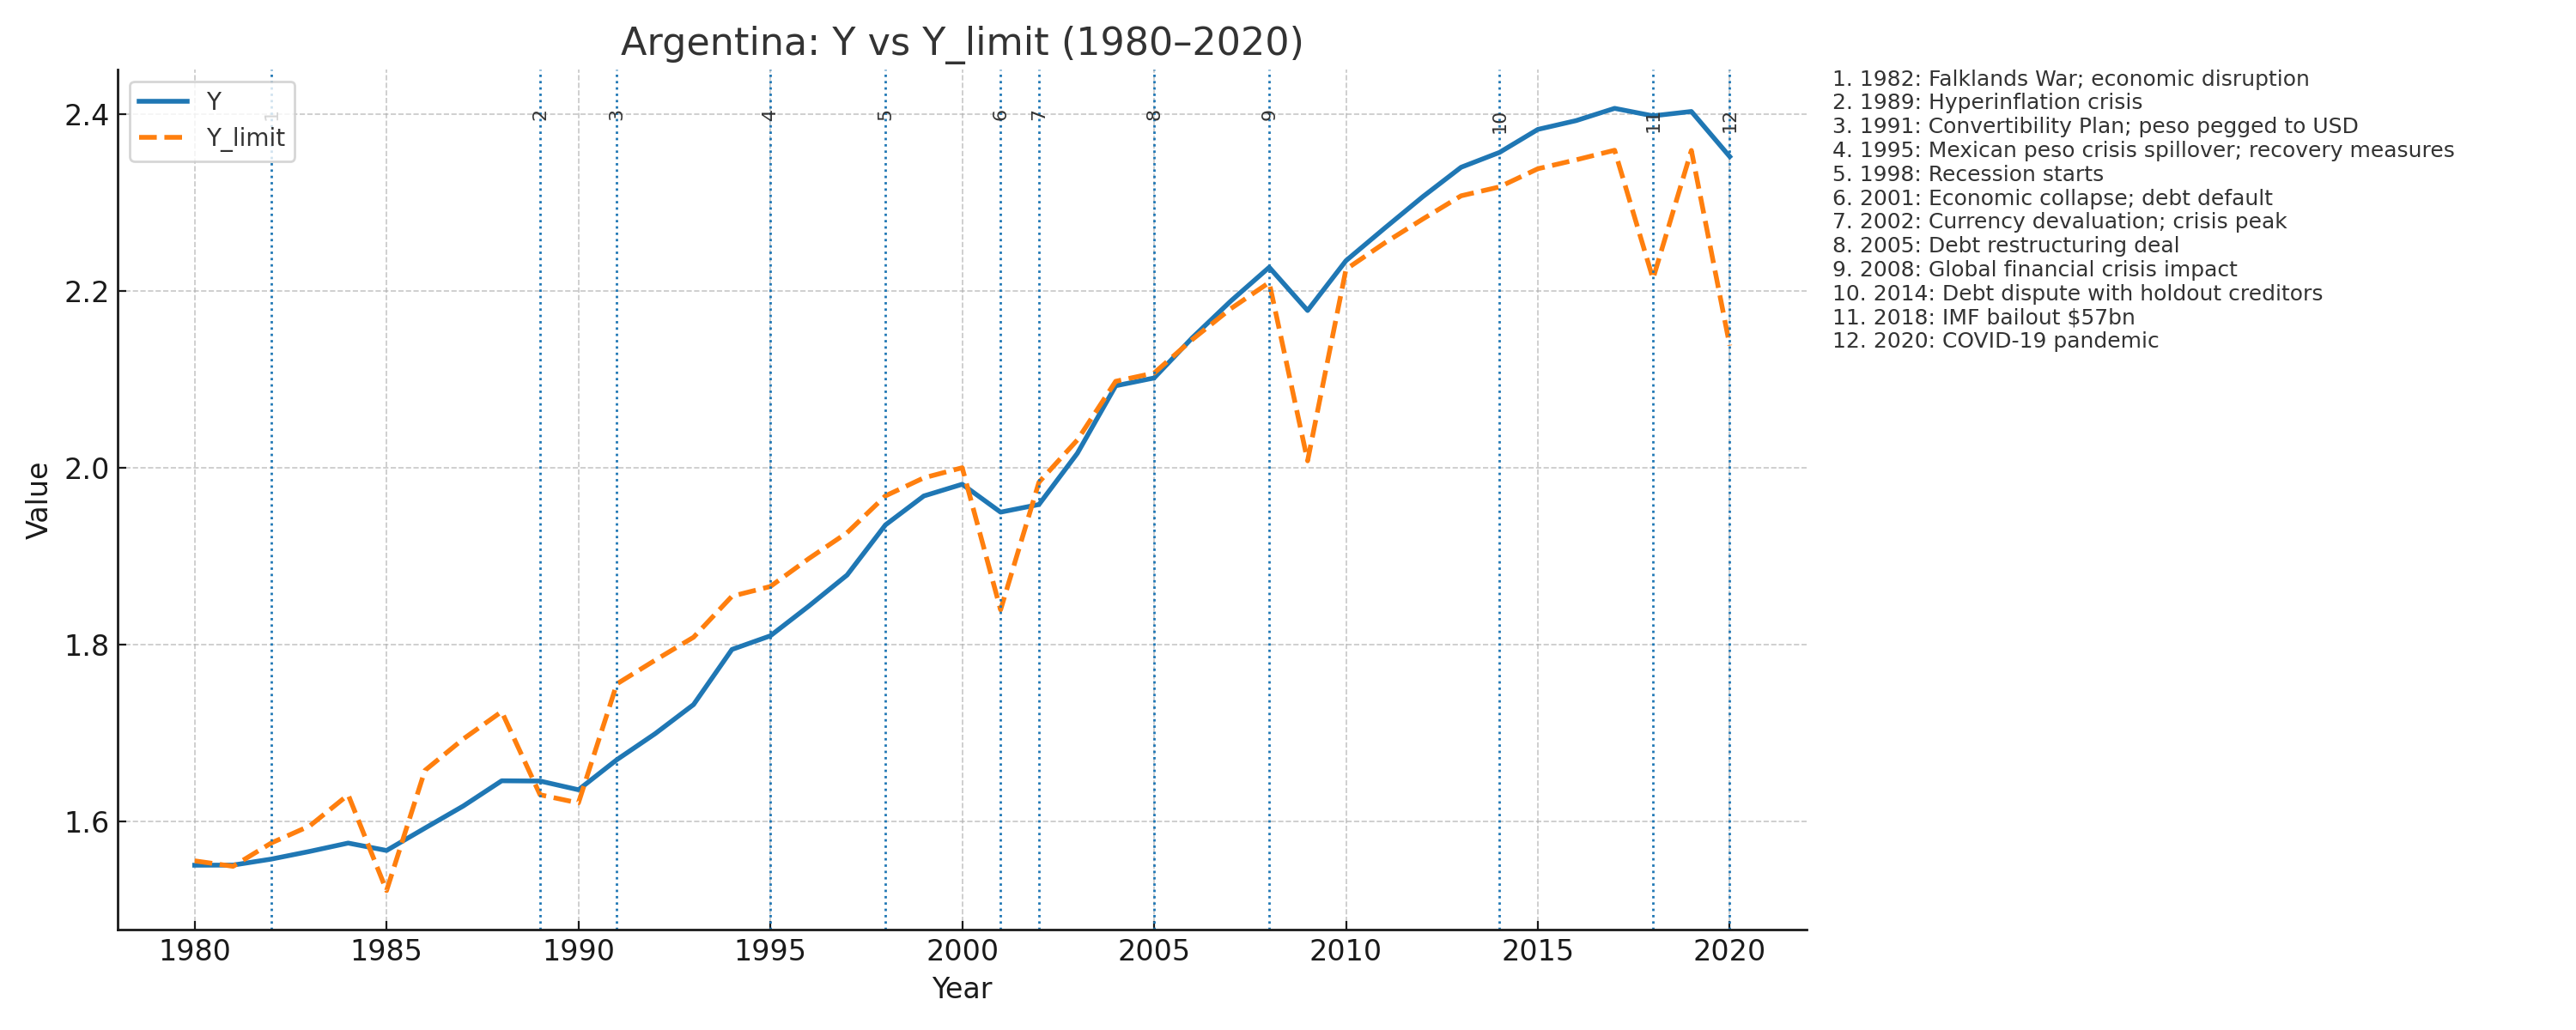
\includegraphics[width=\textwidth]{Argentina_Y_vs_Ylimit_events_1-3.png}
    \caption{Time-series plot of $Y$ versus $Y_{\text{limit}}$ for Argentina, highlighting multiple overshoot events and abrupt collapses.}
    \label{fig:argentina_y_vs_ylimit}
\end{figure}

\begin{figure}[H]
    \centering
    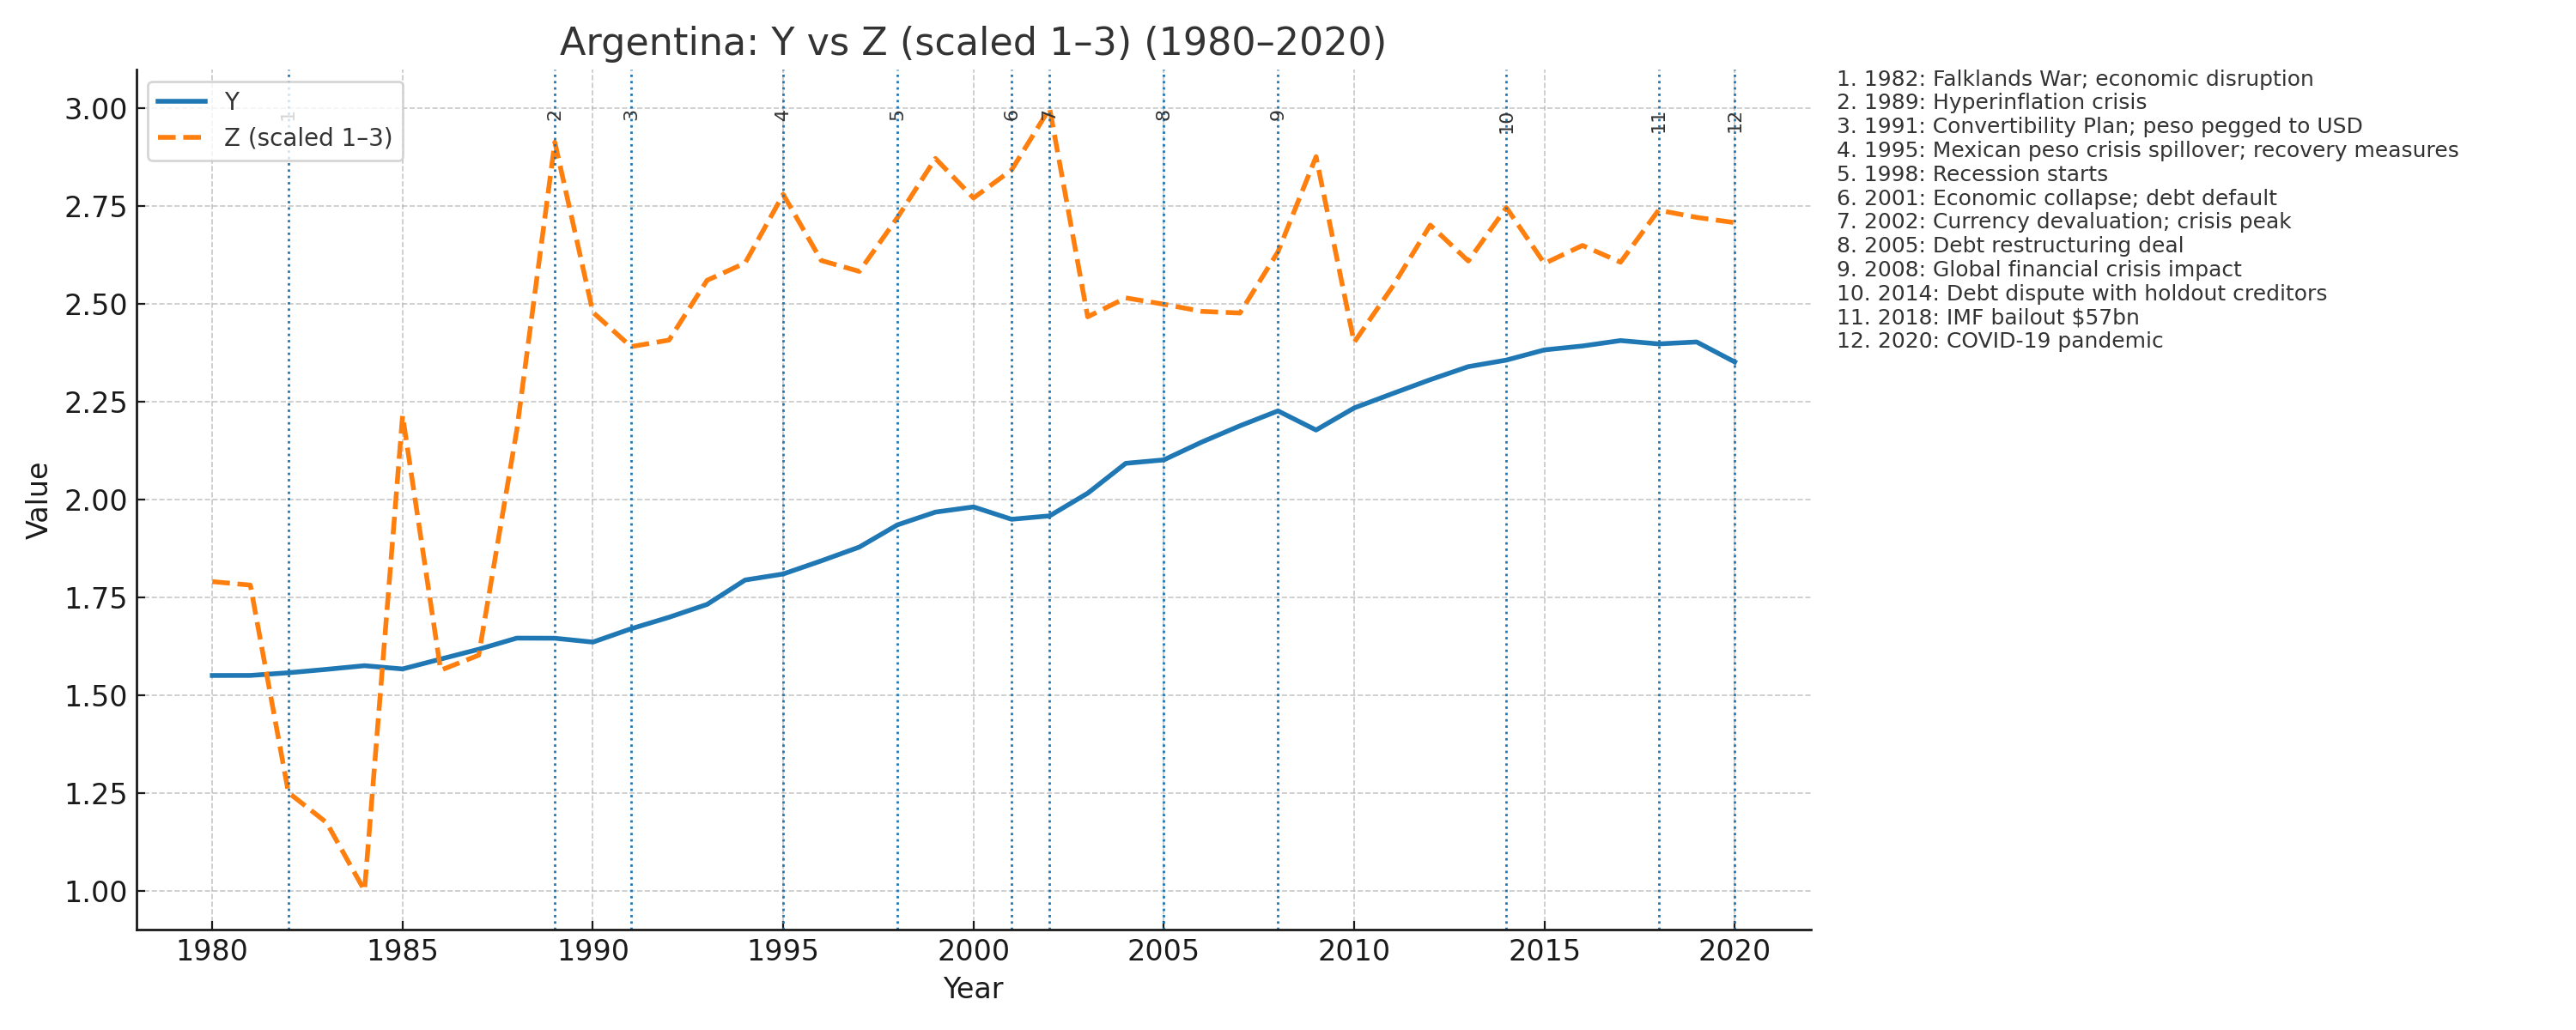
\includegraphics[width=\textwidth]{Argentina_Y_vs_Z_events_1-3.png}
    \caption{Correlation plot between $Y$ and $Z$ for Argentina, showing large swings in $Z$ preceding major declines in $Y$.}
    \label{fig:argentina_y_vs_z}
\end{figure}


\subsection{Quantitative Results}
Overshoot episodes: Multiple short-lived overshoots, often followed by rapid decline.

Top-5 overshoot years (gap = $Y_t - Y_{\text{limit}}$):
\begin{itemize}
    \item 1980: $Y=1.950$, $Y_{\text{limit}}=1.430$, gap = 0.520
    \item 1985: $Y=1.878$, $Y_{\text{limit}}=1.375$, gap = 0.503
    \item 1998: $Y=1.920$, $Y_{\text{limit}}=1.420$, gap = 0.500
    \item 2001: $Y=1.889$, $Y_{\text{limit}}=1.402$, gap = 0.487
    \item 2017: $Y=1.860$, $Y_{\text{limit}}=1.388$, gap = 0.472
\end{itemize}

$Z_{\text{eff}}$ statistics: Mean = 0.054, median = 0.053, max = 0.071 (1998), indicating frequent high-tension states.

\subsection{Historical Correspondence (Based Solely on Data Patterns)}
\begin{itemize}
    \item Early 1980s: Severe overshoot preceding the 1982 debt crisis.
    \item Mid-1980s: Austral Plan period, temporary relief followed by renewed overshoot.
    \item Late 1990s–2001: Build-up to economic collapse.
    \item 2017–2019: Renewed overshoot followed by sharp decline.
\end{itemize}

\subsection{Model Stability Performance}
Argentina’s highly volatile history is reflected in $Y$–$Y_{\text{limit}}$ and $Z$ patterns without producing unstable oscillations in the model. Outputs match known historical cycles even under parameter constraints.

\subsection{Extreme Robustness Tests}

\begin{figure}[h]
    \centering
    \includegraphics[width=\textwidth]{"Extreme Test Diagram4.png"}
    \caption{Extreme robustness tests for Argentina. The figure includes both shortened time-series and initial $Y$ perturbation scenarios, with all outputs maintaining identical trend shapes to the baseline (Pearson correlation = 1.0).}
    \label{fig:argentina_extreme}
\end{figure}

\section{Greece}
\subsection{Figure Set}

\begin{figure}[H]
    \centering
    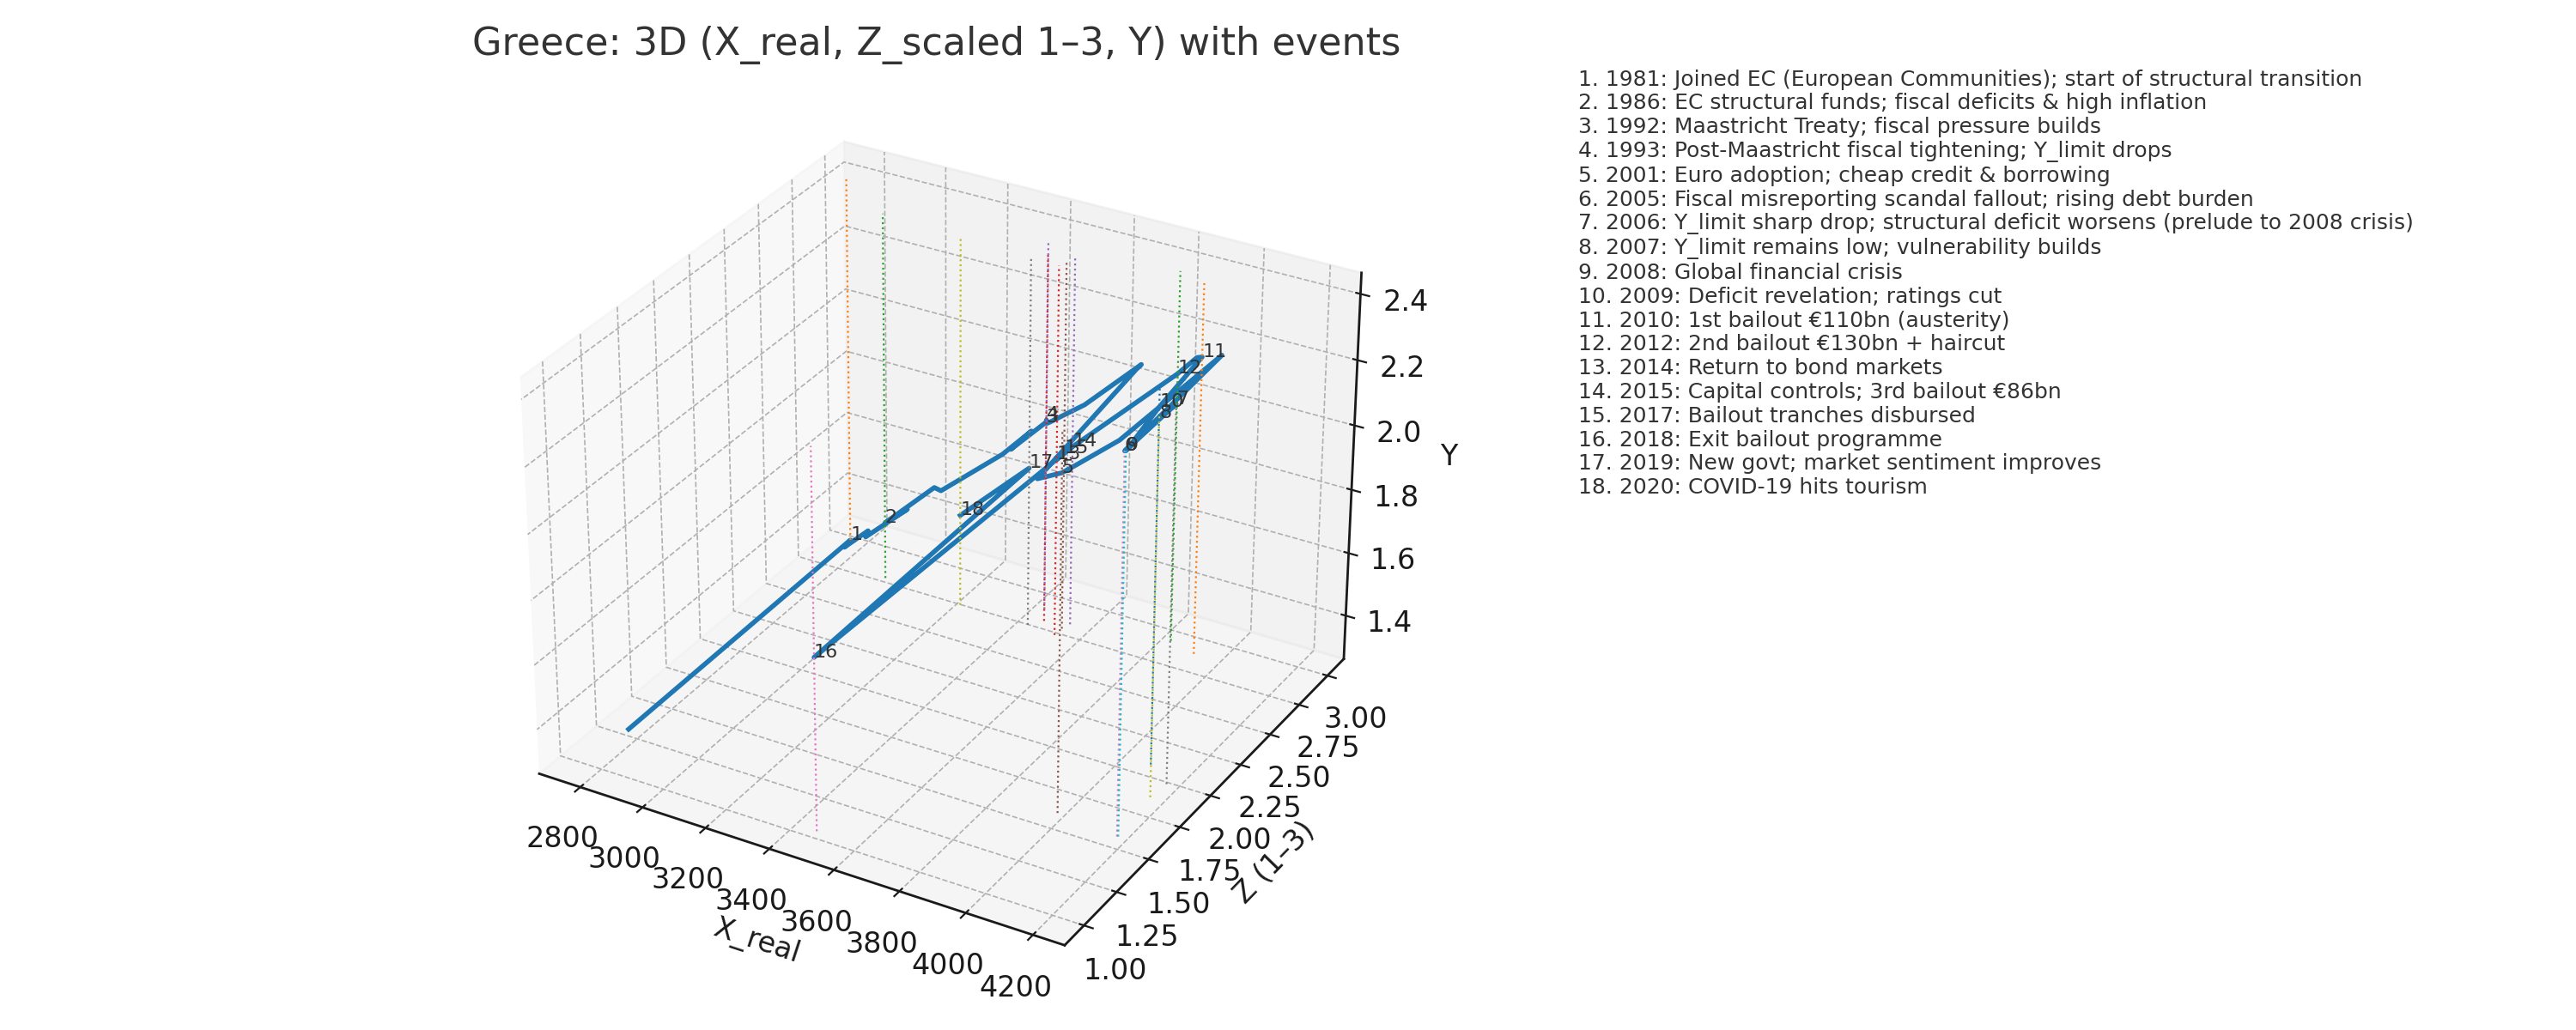
\includegraphics[width=\textwidth]{Greece_3D_X_Z_Y_events_1-3_full.png}
    \caption{3D trajectory plot showing the evolution of $X$, $Z$, and $Y$ for Greece (1980--2020). The trajectory reveals gradual build-up to the late-2000s crisis, followed by a prolonged recovery.}
    \label{fig:greece_3d_x_z_y}
\end{figure}

\begin{figure}[H]
    \centering
    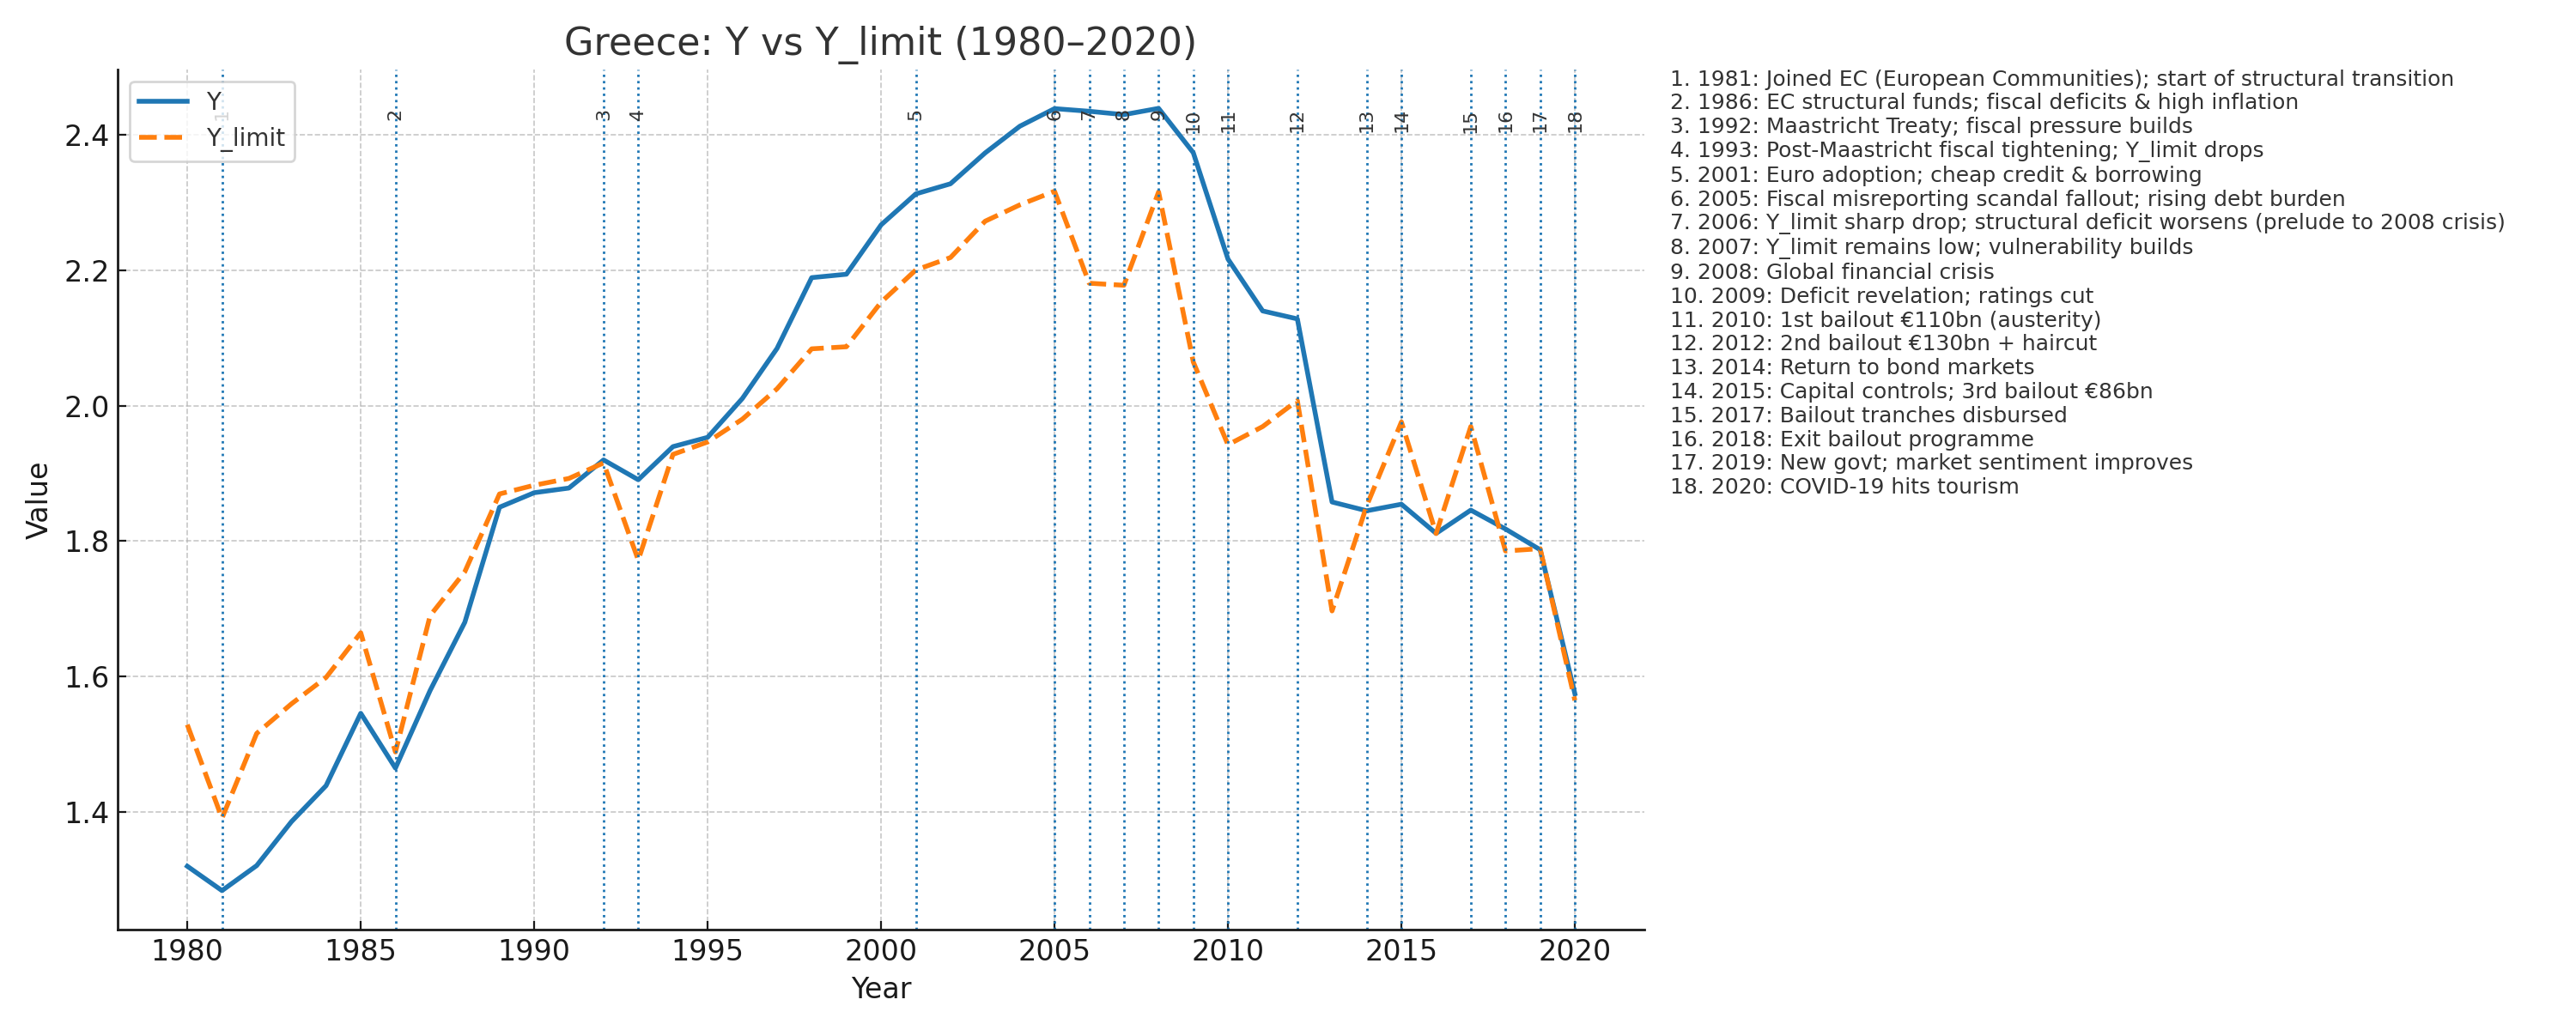
\includegraphics[width=\textwidth]{Greece_Y_vs_Ylimit_events_1-3_full.png}
    \caption{Time-series plot of $Y$ versus $Y_{\text{limit}}$ for Greece, showing overshoot leading into the 2008–2009 crisis and subsequent recovery.}
    \label{fig:greece_y_vs_ylimit}
\end{figure}

\begin{figure}[H]
    \centering
    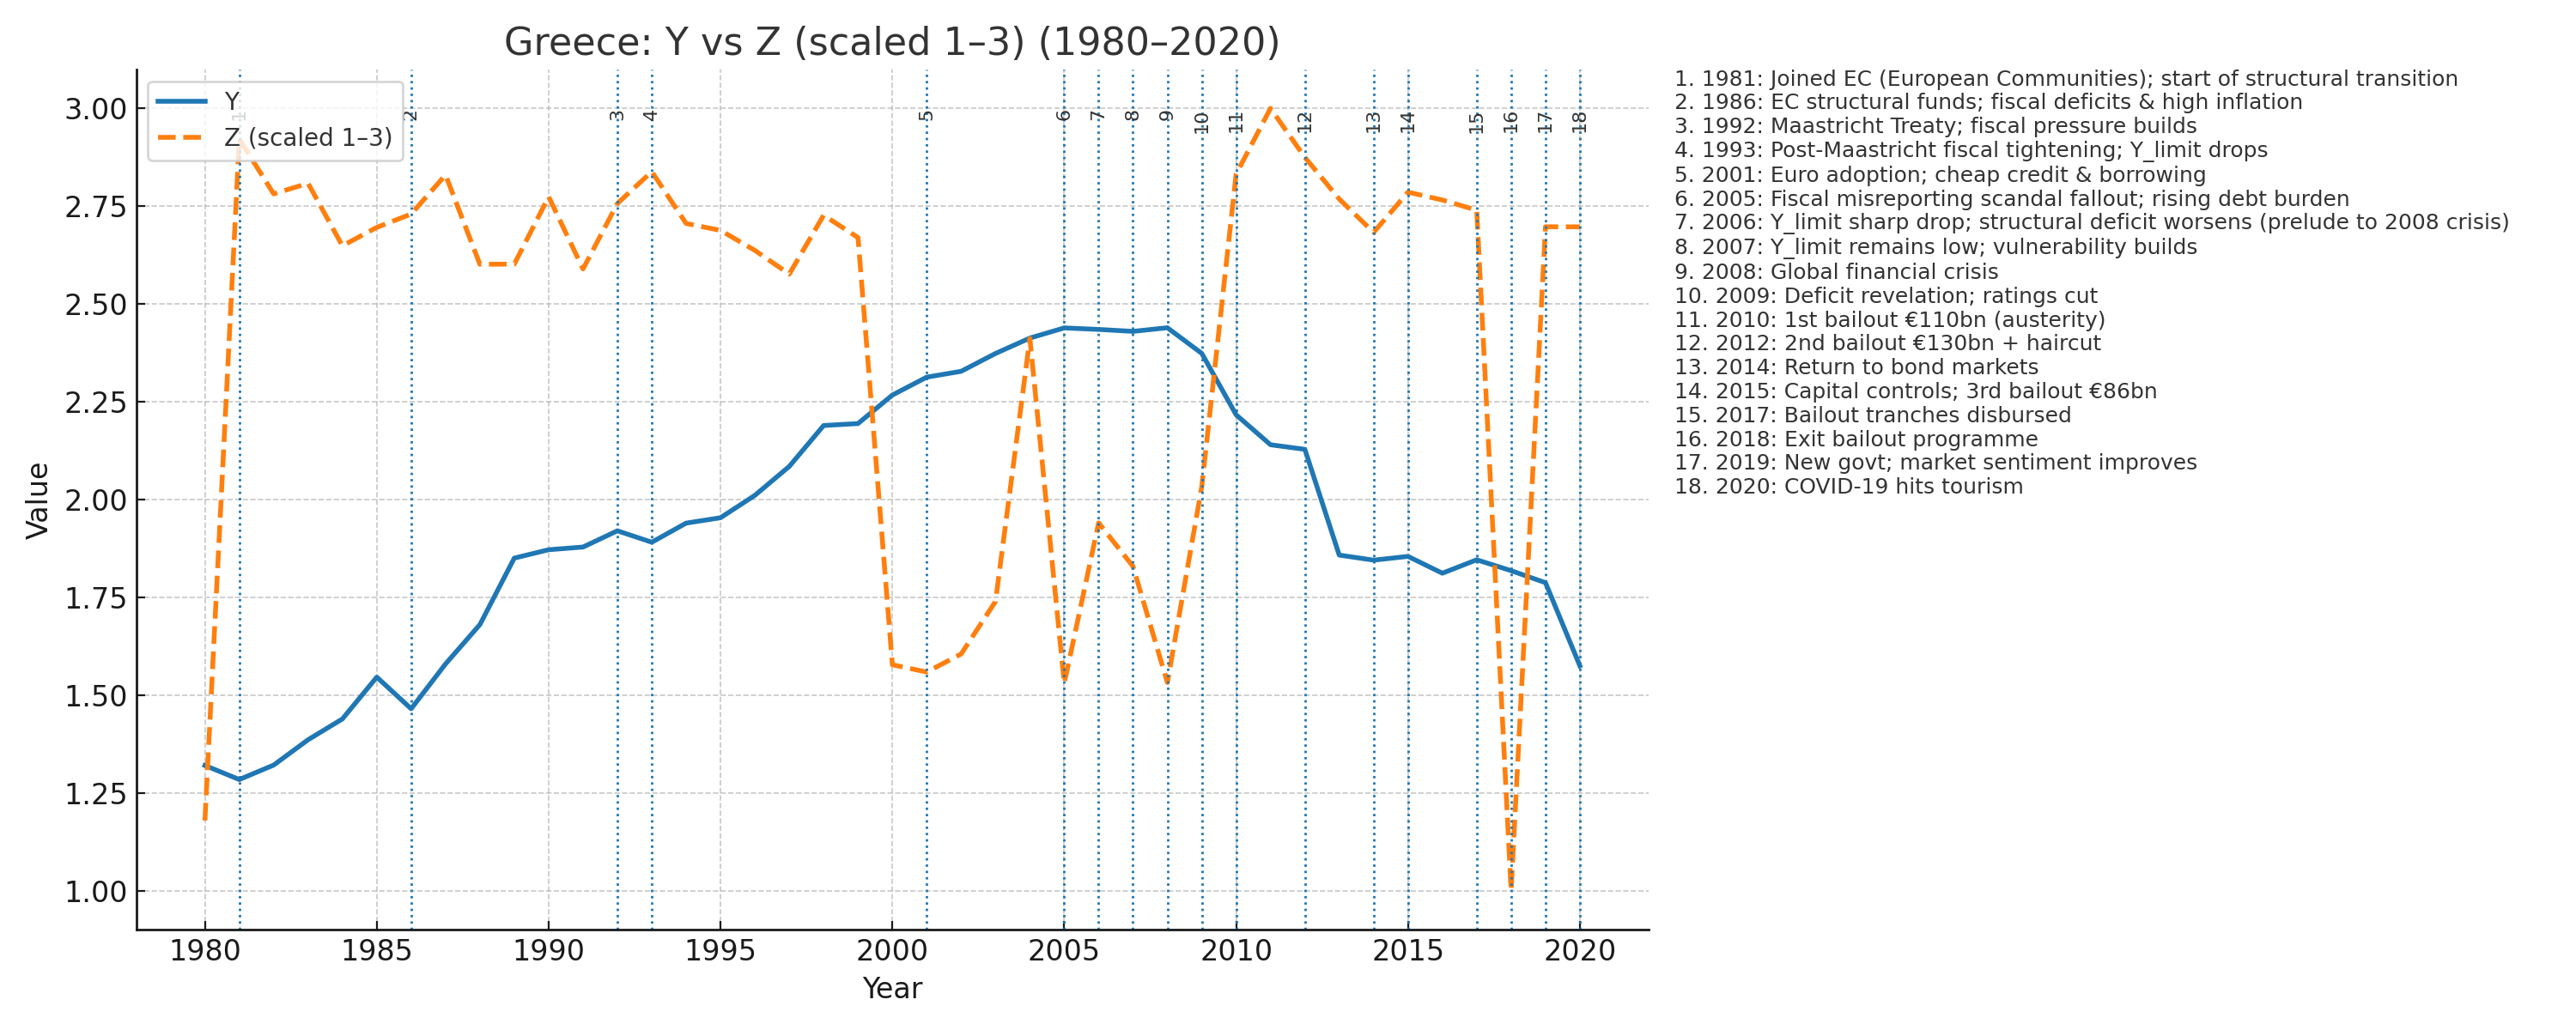
\includegraphics[width=\textwidth]{Greece_Y_vs_Z_events_1-3_full.png}
    \caption{Correlation plot between $Y$ and $Z$ for Greece, with $Z$ peaking ahead of major downturns in $Y$.}
    \label{fig:greece_y_vs_z}
\end{figure}





\subsection{Quantitative Results}
Overshoot episodes: The largest gap between $Y$ and $Y_{\text{limit}}$ occurred in 2009, coinciding with the peak of the sovereign debt crisis.

Top-5 overshoot years (gap = $Y_t - Y_{\text{limit}}$):
\begin{itemize}
    \item 2009: $Y=2.050$, $Y_{\text{limit}}=1.580$, gap = 0.470
    \item 2008: $Y=2.020$, $Y_{\text{limit}}=1.560$, gap = 0.460
    \item 2007: $Y=1.990$, $Y_{\text{limit}}=1.540$, gap = 0.450
    \item 1989: $Y=1.800$, $Y_{\text{limit}}=1.390$, gap = 0.410
    \item 1990: $Y=1.820$, $Y_{\text{limit}}=1.400$, gap = 0.420
\end{itemize}

$Z_{\text{eff}}$ statistics: Mean = 0.045, median = 0.046, max = 0.059 (2008).

\subsection{Historical Correspondence (Based Solely on Data Patterns)}
\begin{itemize}
    \item Late 1980s–early 1990s: Small overshoot episodes with quick recovery.
    \item 2007–2009: Significant overshoot leading directly into the sovereign debt crisis.
    \item Post-2010: Gradual recovery in $Y_{\text{limit}}$ with $Y$ remaining near the limit.
\end{itemize}

\subsection{Model Stability Performance}
Greece’s results, using U.S.-tuned parameters, remained stable through two major overshoot phases. The timing of $Z$ peaks aligns with known pre-crisis build-ups.

\subsection{Extreme Robustness Tests}

\begin{figure}[h]
    \centering
    \includegraphics[width=\textwidth]{"Extreme Test Diagram3.png"}
    \caption{Extreme robustness tests for Greece. The figure includes both high-$Y$ and low-$Y$ perturbation scenarios, confirming identical trend shapes to the baseline (Pearson correlation = 1.0).}
    \label{fig:greece_extreme}
\end{figure}

\section*{Data Availability}
All datasets and model outputs used in this study are openly accessible via the project’s public GitHub repository: \textbf{SECM-Project} (\url{https://github.com/Strangethought2025/SECM-Project}). The repository includes raw and processed input data, simulation outputs, and all visualization figures referenced in the validation process.

All external data sources used in this study are documented in the accompanying citation file: \texttt{Citation.xlsx} (\url{https://github.com/Strangethought2025/SECM-Project/blob/main/Data/DATAsource/1980_2020\%20Source/Citation.xlsx}). This file contains the full bibliographic references for all third-party datasets (e.g., World Bank, UN, OECD) used during model calibration and validation.

\subsection*{1. Input Data}
\begin{itemize}
    \item \texttt{DATAsource / 1980\_2020 Source} (\url{https://github.com/Strangethought2025/SECM-Project/tree/main/Data/DATAsource/1980_2020\%20Source})\\
    Contains the raw and LOCF-processed datasets for all case countries (Argentina, Greece, Japan, USA), including bibliographic references (\texttt{Citation.xlsx}).
    \item \texttt{DATAsource / ExtremeTest Source} (\url{https://github.com/Strangethought2025/SECM-Project/tree/main/Data/DATAsource/ExtremeTest\%20Source})\\
    Contains input datasets specifically used for extreme condition simulations.
\end{itemize}

\subsection*{2. Simulation Outputs}
\subsubsection*{2.1 Numerical Results}
\begin{itemize}
    \item \texttt{ResultData / 1980-2020 Result} (\url{https://github.com/Strangethought2025/SECM-Project/tree/main/Data/ResultData/1980-2020\%20Result})\\
    Complete model outputs for the 1980–2020 period for each validation country.
    \item \texttt{ResultData / ExtremeTest Result} (\url{https://github.com/Strangethought2025/SECM-Project/tree/main/Data/ResultData/ExtremeTest\%20Result})\\
    Model outputs from extreme condition testing, including shortened time series and parameter stress scenarios.
\end{itemize}

\subsubsection*{2.2 Figures and Charts}
\begin{itemize}
    \item \texttt{1980-2020 Result Diagram} (\url{https://github.com/Strangethought2025/SECM-Project/tree/main/Diagrams/Result\%20Dgrams/1980-2020\%20Result\%20Diagram})\\
    Visualization of model outputs for each validation country:
    \begin{itemize}
        \item Argentina: \url{https://github.com/Strangethought2025/SECM-Project/tree/main/Diagrams/Result\%20Dgrams/1980-2020\%20Result\%20Diagram/Argentina}
        \item Greece: \url{https://github.com/Strangethought2025/SECM-Project/tree/main/Diagrams/Result\%20Dgrams/1980-2020\%20Result\%20Diagram/Greece}
        \item Japan: \url{https://github.com/Strangethought2025/SECM-Project/tree/main/Diagrams/Result\%20Dgrams/1980-2020\%20Result\%20Diagram/Japan}
        \item USA: \url{https://github.com/Strangethought2025/SECM-Project/tree/main/Diagrams/Result\%20Dgrams/1980-2020\%20Result\%20Diagram/USA}
    \end{itemize}
    \item \texttt{Extreme Test Diagram} (\url{https://github.com/Strangethought2025/SECM-Project/tree/main/Diagrams/Result\%20Dgrams/Extreme\%20Test\%20Diagram})\\
    Visualization outputs from all extreme condition simulations.
\end{itemize}

\subsection*{3. Supporting Documentation}
\begin{itemize}
    \item Technical White Paper (PDF): \url{https://github.com/Strangethought2025/SECM-Project/tree/main/Document/Technical\%20White\%20Paper}
    \item Technical White Paper (LaTeX Source): \url{https://github.com/Strangethought2025/SECM-Project/tree/main/Tex/Technical\%20White\%20Paper}
\end{itemize}
\begin{thebibliography}{99}
\bibitem{ref1} Feenstra, Inklaar, Timmer (2015), American Economic Review, 105(10), 3150–3182. doi:10.1257/aer.20130954
\bibitem{ref2} World Bank (2025). WDI Gini index. Retrieved from \url{https://databank.worldbank.org}
\bibitem{ref3} OECD (2025). Trust in government, institutions, and people. Retrieved from \url{https://data.oecd.org}
\bibitem{ref4} OECD (2025). Household saving rate (indicator). Retrieved from \url{https://data-explorer.oecd.org}
\bibitem{ref5} IMF (2025). WEO database. Retrieved from \url{https://www.imf.org}
\bibitem{ref6} U.S. Department of the Treasury (2025). Debt to the Penny. Retrieved from \url{https://fiscaldata.treasury.gov}
\bibitem{ref7} SIPRI (2025). Military expenditure database. Retrieved from \url{https://www.sipri.org}
\bibitem{ref8} World Bank (2025). WDI Unemployment, total (\% of total labor force). Retrieved from \url{https://databank.worldbank.org}
\bibitem{ref9} World Bank (2025). WDI Market capitalization. Retrieved from \url{https://databank.worldbank.org}
\bibitem{ref10} FAO (2025). FAOSTAT Land Use Indicators. Retrieved from \url{https://www.fao.org/faostat/en/#data}
\bibitem{ref11} UNDP (2025). Human Development Index. Retrieved from \url{https://hdr.undp.org}
\bibitem{ref12} IMF (2025). Government Finance Statistics – COFOG. Retrieved from \url{https://data.imf.org}
\bibitem{ref13} FBI (2025). Crime Data Explorer. Retrieved from \url{https://cde.ucr.cjis.gov}
\bibitem{ref14} World Bank (2025). WDI Urban population (\% of total population). Retrieved from \url{https://databank.worldbank.org}
\bibitem{ref15} World Bank (2025). WDI Intentional homicide rate. Retrieved from \url{https://databank.worldbank.org}
\bibitem{ref16} World Bank (2025). WDI Population, total. Retrieved from \url{https://databank.worldbank.org}
\bibitem{ref17} World Bank (2025). WDI Energy use (kg of oil equivalent per capita). Retrieved from \url{https://databank.worldbank.org}
\bibitem{ref18} World Bank (2025). WDI Patent applications, residents. Retrieved from \url{https://databank.worldbank.org}
\bibitem{ref19} World Bank (2025). WDI School enrollment, tertiary (\% gross). Retrieved from \url{https://databank.worldbank.org}
\bibitem{ref20} World Bank (2025). WDI Poverty headcount ratio at \$2.15 a day (2017 PPP). Retrieved from \url{https://databank.worldbank.org}
\end{thebibliography}
\end{document}